\documentclass[notitlepage,11pt, a4paper]{article}
\usepackage[utf8]{inputenc}

\usepackage{amsfonts, amssymb, amsmath}
\usepackage{mathtools}

\usepackage{graphicx}

\usepackage{caption}
\usepackage{subcaption}

\usepackage[colorlinks=true, pdfstartview=FitV, linkcolor=blue, citecolor=blue, urlcolor=blue,pagebackref=false]{hyperref}
\usepackage{varioref}
\usepackage[capitalize]{cleveref}

% BIBLIOGRAPHY MANAGEMENT

\usepackage[numbers]{natbib}
\bibliographystyle{plainnat}


% PAGE DIMENSIONS

\topmargin -0.5in
\textheight 9 in
\oddsidemargin 0.15in
\evensidemargin 0.25in
\textwidth 6.15in
\parskip=5pt
% THEOREM ENVIRONMENTS

\usepackage{amsthm}
\usepackage{thmtools}

\declaretheorem[numberwithin=section]{theorem}
\declaretheorem[sibling=theorem]{lemma}
\declaretheorem[sibling=theorem]{corollary}
\declaretheorem[sibling=theorem]{proposition}
\declaretheorem[sibling=theorem]{remark}
\declaretheorem[sibling=theorem]{definition}

% COMMENT ENVIRONMENTS

\usepackage{xcolor}
\definecolor{darkred}{rgb}{0.9,0.1,0.1}
\newcommand\comment[1]{\marginpar{\raggedright\scriptsize{\textcolor{darkred}{#1}}}}
\newcommand\myworries[1]{\textcolor{red}{[#1]}}

%%%%%%%%%% ABBREVIATIONS

% BLACKBOARD BOLD

\def \C {{\mathbb C}}
\def \D {{\mathbb D}}
\def \E {{\mathbb E}}
\def \N {{\mathbb N}}
\def \P {{\mathbb P}}
\def \Q {{\mathbb Q}}
\def \R {{\mathbb R}}
\def \Z {{\mathbb Z}}
\def \T {{\mathbb T}}
\def \I {{\mathbb I}}
\def \T {{\mathbb T}}

% MATHCAL

\def \cA {{\mathcal A}}
\def \cC {{\mathcal C}}
\def \cD {{\mathcal D}}
\def \cE {{\mathcal E}}
\def \cF {{\mathcal F}}
\def \cG {{\mathcal G}}
\def \cH {{\mathcal H}}
\def \cI {{\mathcal I}}
\def \cJ {{\mathcal J}}
\def \cK {{\mathcal K}}
\def \cL {{\mathcal L}}
\def \cM {{\mathcal M}}
\def \cN {{\mathcal N}}
\def \cO {{\mathcal O}}
\def \cP {{\mathcal P}}
\def \cQ {{\mathcal Q}}
\def \cR {{\mathcal R}}
\def \cS {{\mathcal S}}
\def \cT {{\mathcal T}}

% VECTORS

\def \vD {{\mathbf D}}
\def \vX {{\mathbf X}}
\def \vZ {{\mathbf Z}}
\def \va {{\mathbf a}}
\def \vc {{\mathbf c}}
\def \vd {{\mathbf d}}
\def \vk {{\mathbf k}}
\def \vs {{\mathbf s}}
\def \vu {{\mathbf u}}
\def \vx {{\mathbf x}}
\def \vy {{\mathbf y}}

% MAKING SUBSET AND SUPSET BY DEFAULT SUBSETEQ AND SUPSETEQ

\def \subset {\subseteq}
\def \supset {\supseteq}

% PAIRED DELIMITERS

\DeclarePairedDelimiter{\abs}{\lvert}{\rvert}
\DeclarePairedDelimiter{\norm}{\lVert}{\rVert}
\DeclarePairedDelimiter{\floor}{\lfloor}{\rfloor}

% MATH OPERATORS

\DeclareMathOperator{\var}{Var}
\DeclareMathOperator{\cov}{Cov}
\DeclareMathOperator{\corr}{Corr}
\DeclareMathOperator{\iso}{Iso}

% MISC SYMBOLS

\def\one{\rlap{\mbox{\small\rm 1}}\kern.15em 1} % indicator function

% CONVERGENCE
\def \todist {\xrightarrow[]{\mathrm{(d)}}}
\def \toas {\xrightarrow[]{\mathrm{a.s.}}}

% PROJECT SPECIFIC SYMBOLS

\usepackage{stmaryrd} % needed for double square brackets
\DeclarePairedDelimiter{\pathbtw}{\llbracket}{\rrbracket}
\def \littleo {o}
\def \bigo {\mathcal O}
\newcommand \diff[2] {\frac{\mathrm{d}#1}{\mathrm{d}#2}}
\newcommand*\dif{\mathop{}\!\mathrm{d}}
\def \lattice {\Lambda}
\newcommand \vectwo[2] {\begin{pmatrix} #1 \\ #2 \end{pmatrix}}
\def \omegaevent {\mathcal E}
\def \maxeval {{\lambda_{\text{max}}}}
\def \mineval {{\lambda_{\text{min}}}}
\def \centeredX {\hat{\vX}}
\def \distmdm {d_{\vec{G}}}

%%%%%%%%%%%%%%

\title{Universality for the directed configuration model with random degrees: metric space convergence of the strongly connected components at criticality}
\author{Serte Donderwinkel and Zheneng Xie}
\date{Version: \today}

\begin{document}

\maketitle
\begin{abstract}
  We consider the strongly connected components (SCC) of a uniform directed graph on $n$ vertices with i.i.d. degree tuples distributed as $(D^-,D^+)$, with $\E[D^+]=\E[D^-]=\mu$. We condition on the total in-degree and total out-degree to be equal. A phase transition for the emergence of a giant strongly connected component, that contains a positive proportion of the vertices, is known to occur at the critical value $\E[D^-D^+]/\mu=1$. We study the model at this critical value, and additionally, require that $\E[(D^-)^i(D^+)^j]<\infty$ for all $i+j\leq 3$, and for $i=3$, $j=1$. We show that, under these conditions, the strongly connected components ranked by decreasing order of size and rescaled by $n^{-1/3}$, converge in distribution to a sequence of finite strongly connected directed multigraphs with edge lengths which are either $3$-regular or loops. The limit objects are in a $3$-parameter family, which contains the scaling limit of the SCC in the directed Erd\H{o}s-Renyi model at criticality as found in \cite{goldschmidtScalingLimitCritical2019}. This shows that the limit object is universal, and makes this the first universality result for directed graph models. Moreover, this is the first time result on the directed configuration model at criticality. As a trivial consequence, the largest strongly connected components at criticality contain $O(n^{1/3})$ vertices with high probability, and the diameter of the directed graph at criticality is $\Omega(n^{1/3})$ with high probability; two results that were previously unknown.  We use a metric on the space of such multigraphs in which two multigraphs are close if there are compatible isomorphisms between their vertex and edge sets which roughly preserves the edge lengths. We use the product topology on the sequence of multigraphs. Our method involves depth-first exploration of the directed graph, resulting in a spanning forest, of which we study the limit under rescaling.
\end{abstract}
% \tableofcontents
\section{Introduction}


\subsection{Overview}

Edges in real-world networks are often directed, such as links on the world wide web, follows on Twitter or disease transmission. When analysing networks a natural quantity to consider is are the degrees of nodes in the network.  In this paper we will consider sampling an i.i.d.\ sequence of in- and out-degrees. Conditional on the total in-degree being equal to the total out-degree, we will sample a uniform directed graph (digraph) with the given degree sequence. Results on such graphs provide insight into what additional structure a real-world network has beyond it's degree sequence.

When considering such models, previous work by \citet{cooperSizeLargestStrongly2004} shows that there is a phase transition in the directed connectivity of the graph. Below some threshold, each of the strongly connected components of the graph will contain a negligible proportion of vertices in the graph whereas above the threshold there will exist a unique strongly connected component that occupies a positive proportion of the vertices.  We will study the behaviour of the model at criticality, specifically that there exists a sequence of random weighted directed multigraphs that can be understood as the scaling limit of the strongly connected components when viewed in decreasing order of size.

\subsection{Graph theory}

\begin{figure}
    \centering
    \includegraphics[scale=0.6]{Content/Pictures/biggraph2.pdf}
    \caption{A directed graph on [17]. The strongly connected components have vertex sets $\{1,2,5,17\}$, $\{3,6,8,9,14,16\}$, $\{7,11\}$, $\{4\}$, $\{10\}$, $\{12\}$, $\{13\}$, and $\{15\}$. Source figure: \cite{goldschmidtScalingLimitCritical2019}}
    \label{fig.SCCs}
\end{figure}

There are two notions of connectivity when working with a directed graph - weak and strong connectivity. We will be working with the strong notation. We say a vertex $v$ leads to a vertex $w$ if there exists a directed path from $v$ to $w$ in the graph. We say $v$ is strongly connected to $w$ if $v$ leads to $w$ and $w$ leads to $v$. A graph is strongly connected if any pair of vertices in the graph are strongly connected. The relation is an equivalence relation. The digraphs induced by the equivalence classes of are referred to as the strongly connected components (SCCs).

\subsection{Description of the model}

We consider $n$ vertices, to each of which we assign an in-degree and an out-degree. The degree tuples are independent and identically distributed with law $\nu$. For each $i\in [n]$, let $\mathbf{D}_i=(D^-_i,D^+_i)$ be the in- and out-degree of vertex $i$. In order for a graph with this degree sequence to exist, we require that $\sum_{i=1}^n D^-_i=\sum_{i=1}^n D^+_i$, so we will condition on this event. Conditional on $(\mathbf{D}_1,\dots,\mathbf{D}_n)$, sample a uniform digraph with this degree sequence. Denote resulting random digraph by $\vec{G}_n(\nu)$. We are interested in the limit under scaling of the strongly connected components of $\vec{G}_n(\nu)$ as $n\to \infty$.

We require the degree distribution to satisfy the following properties.

\begin{enumerate}
    % \item $\E[(D^-) + D^+)^3] < \infty$
    \item $\E[(D^-)^i(D^+)^j]< \infty$ for $1 \leq i+j\leq 3$ and for $\{i,j\}=\{1,3\}$
    \item $\E[D^-] = \E[D^+]$.
    \item \myworries{lattice condition}
\end{enumerate}

The first condition is required to ensure the steps of a random walk used in the proof has finite variance and thus will convergence (under rescaling) to a Brownian motion.

The second condition and third condition makes sure the event $\{\sum_{i=1}^n D^-_i = \sum_{i=1}^n D^+_i\}$ is well behaved. The second condition ensures this is not a large deviation event and the third condition ensures this event has positive probability for all $n \geq 1$. 

\myworries{go over criticality condition}

We define the following parameters, that will determine the behaviour of the strongly connected components in the limit.
\begin{enumerate}
    \item $\mu:=\E[D^-]=\E[D^+]=\E[D^-D^+]$
    \item $\nu_-:=\frac{\E[(D^-)^2]-\mu}{\mu}$ 
    \item $\sigma_-:=\left(\frac{\mu\E[(D^-)^3]-\E[(D^-)^2]^2}{\mu^2}\right)^{1/2}$ 
    \item $\sigma_+:=\left(\frac{\E[D^-(D^+)^2]-\mu}{\mu}\right)^{1/2}$ 
    \item $\sigma_{-+}:=\frac{\E[(D^-)^2D^+]-\E[(D^-)^2]}{\mu}$ 
\end{enumerate}
% \begin{remark}
% Conditions \ref{cond.beta} and \ref{cond.gamma} ensure that the Central Limit Theorem applies to the fluctuations of the first explored in-degrees around their mean. Condition \ref{cond.critical} ensures that the branching process corresponding to the depth-first exploration (i.e. the exploration of the out-components) is critical. Condition \ref{cond.rho} ensures that this branching process has Brownian scaling. Condition \ref{cond.tau} ensures that the covariance of the in- and out-degrees that are discovered first is finite. Condition \ref{cond.iota} ensures that the strongly connected components are $3$-regular. 
% \end{remark}
\subsection{Metric directed multigraphs and kernels}

\begin{figure}[htbp]
    \centering

    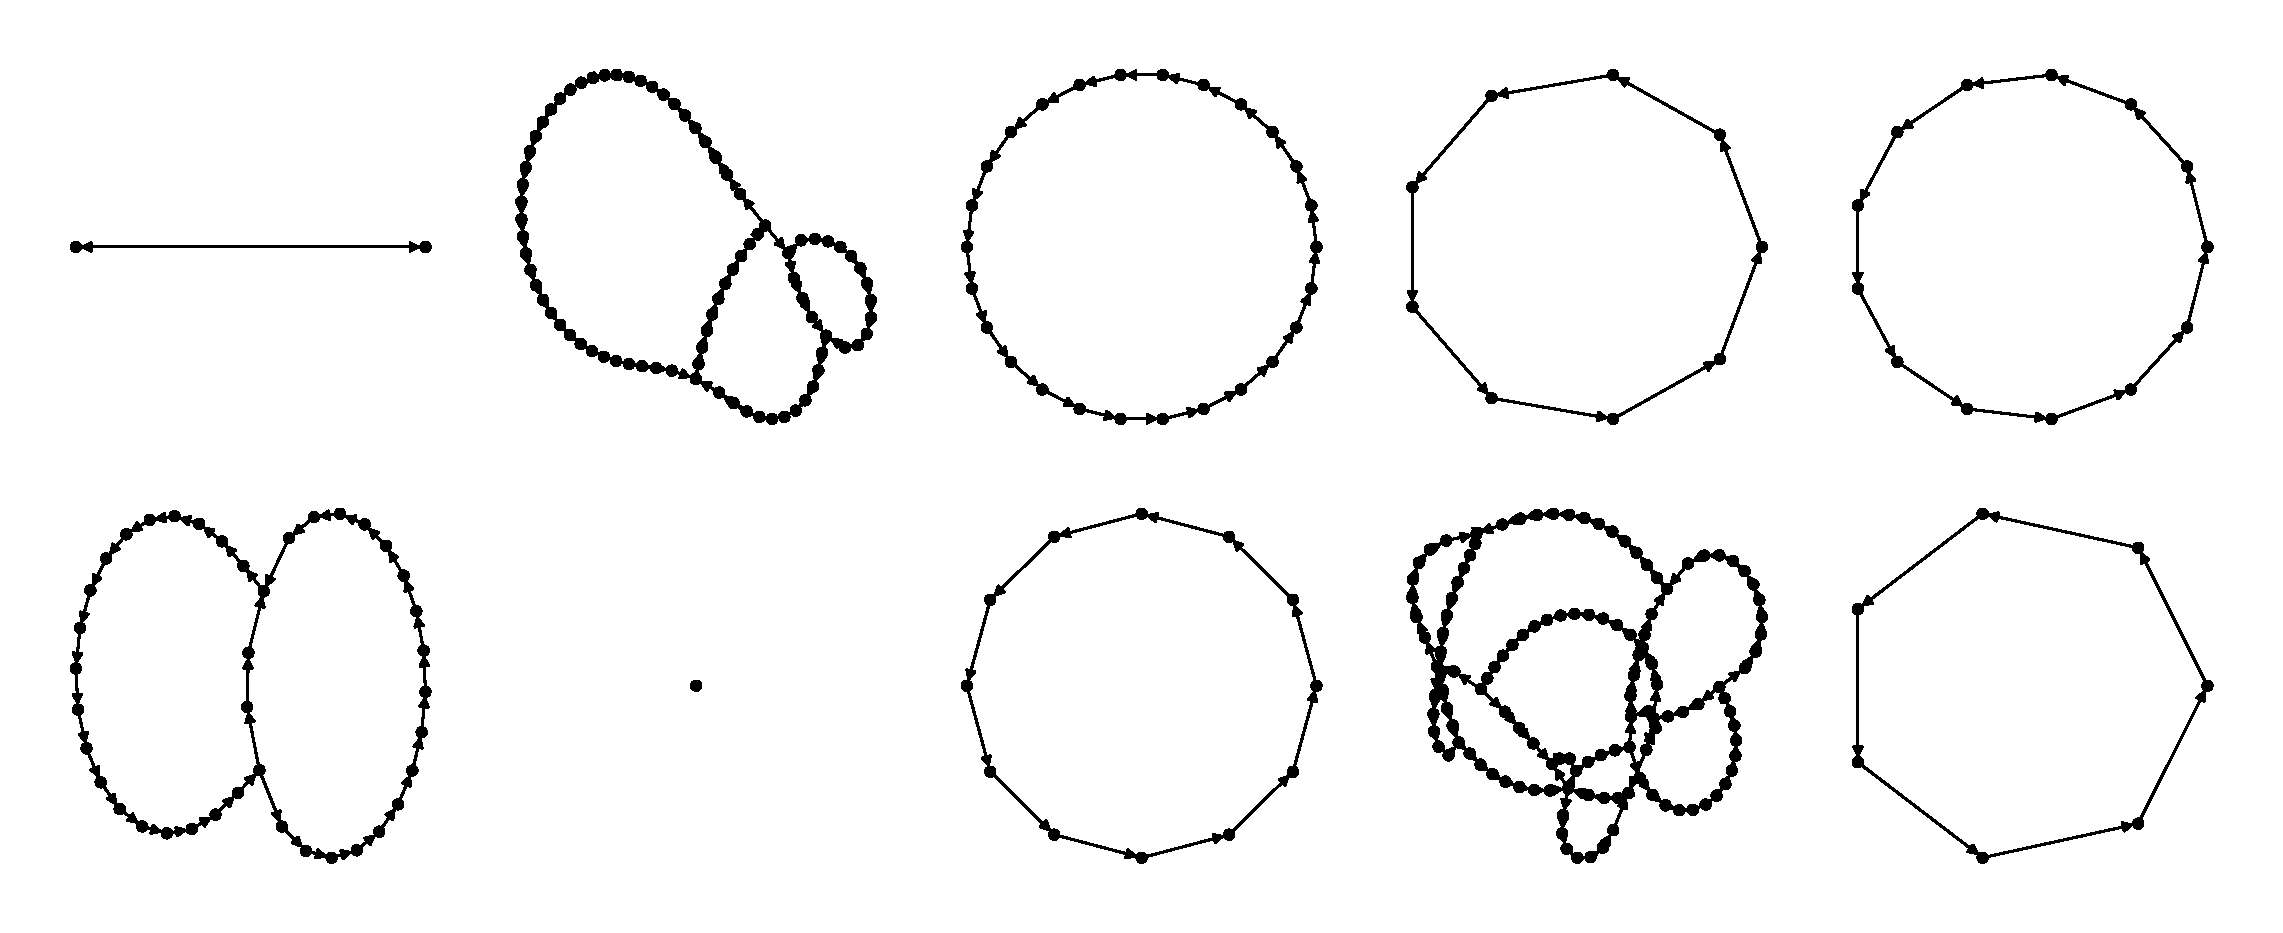
\includegraphics[width=\textwidth]{Content/Pictures/largest_sccs.eps}
    
    \caption{The largest SCC from samples of a directed configuration model with independent $\text{Poisson(1)}$ in- and out-degrees}
    \label{fig:largest-sccs}
\end{figure}

In \cref{fig:largest-sccs} we see the largest SCC from samples of a directed configuration model. As can be seen, while the lengths of paths in the SCC are long, the actual structure of the SCC is often quite simple. Previous work by \citet{goldschmidtScalingLimitCritical2019} shows this is true for the directed Erdős--Renyi model. There it was shown that while the lengths of paths in the SCC will scale like $n^{1/3}$, the actual structure of the SCC will remain finite.

To formalise this idea we will introduce metric directed multigraphs (MDMs). These are simply weighted directed multigraphs, but in our context it is more appropriate to think of the weights as lengths hence the change in naming. Formally a directed multigraph is a tuple $(V, E, r)$ where
\begin{enumerate}
    \item $V$ is a set of vertices,
    \item $E$ is a set of edges, and
    \item $r: E \to V \times V$ is a function mapping edges to their head and tail.
\end{enumerate}
Associated with $r$ are two functions $r_1: E \to V$ and $r_2: E \to V$ such that
\begin{equation*}
    r(e) = (r_1(e), r_2(e))
\end{equation*}
for all $e \in E$. $r_1(e)$ is the tail of the edge $e$ and $r_2(e)$ is the head of the edge $e$. Then a metric directed multigraph (MDM) is a tuple $M = (V, E, r, l)$ where $(V, E, r)$ is a directed multigraph and $l:E \to [0, \infty)$. Let $\zeroloop$ denote the MDM consisting of a single vertex with a self loop of length 0.

An isomorphism between two MDMs $M = (V, E, r, l)$ and $M' = (V', E', r', l)$ is a pair of functions $(i_V, i_E)$ where $i_V: V \to V'$ and $i_E: E \to E'$ are bijections satisfying
\begin{equation*}
    r'(i_E(e)) = (i_V(r_1(e)), i_V(r_2(e)))
\end{equation*}
for all $e \in E$. We say two MDMs are isomorphic if there exists an isomorphism between them. Intuitively this means the MDMS have the same graph structures up to a relabelling of the edges and vertices. Write $\iso(M, M')$ for the set of all isomorphisms between $M$ and $M'$.

We now define a distance $\distmdm$ between two MDMs $M$ and $M'$.  Any isomorphism between $M$ and $M'$ gives a correspondence between the edges of $M$ and the edges of $M'$. We can then take an $\ell_{\infty}$ distance between the lengths of the edges and finally take the isomorphism which minimizes this distance. If $M$ and $M'$ are not isomorphic we can set the distance to be infinite. Formally
\begin{equation*}
    \distmdm(M, M') = \begin{cases}
        \inf_{(i_V, i_E) \in \iso(M, M')} \sup_{e \in E} \abs{l(e) - l(i_E(e))} & \text{if $M$ and $M'$ are isomorphic,} \\
        \infty & \text{otherwise.}
    \end{cases}
\end{equation*}

\begin{figure}[htbp]
    \centering
    \begin{subfigure}[htbp]{0.45\textwidth}
        \centering
        \includegraphics[width=0.95\textwidth]{Content/Pictures/smoothing1.eps}
        \caption{The graph before smoothing $w$}
    \end{subfigure}
    \hfill
    \begin{subfigure}[htbp]{0.45\textwidth}
        \centering
        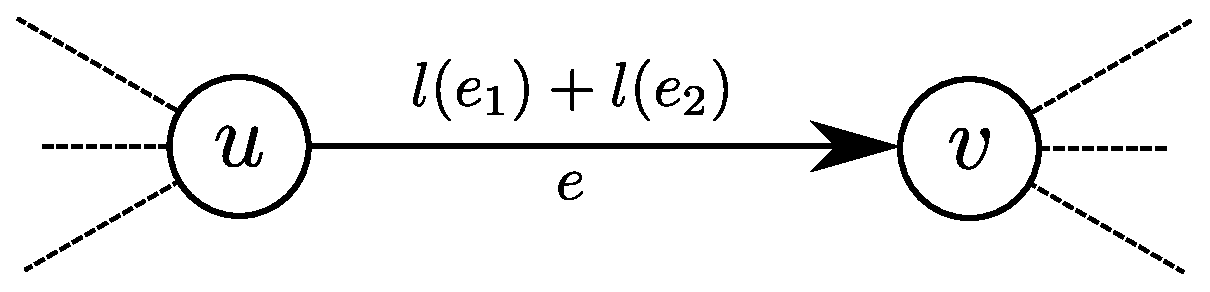
\includegraphics[width=0.95\textwidth]{Content/Pictures/smoothing2.eps}
        \caption{The graph before smoothing $w$}
    \end{subfigure}
    \caption{Smoothing a vertex $w$}
    \label{fig:smoothing}
\end{figure}

\begin{figure}[htbp]
    \centering
    \begin{subfigure}[htbp]{0.45\textwidth}
        \centering
        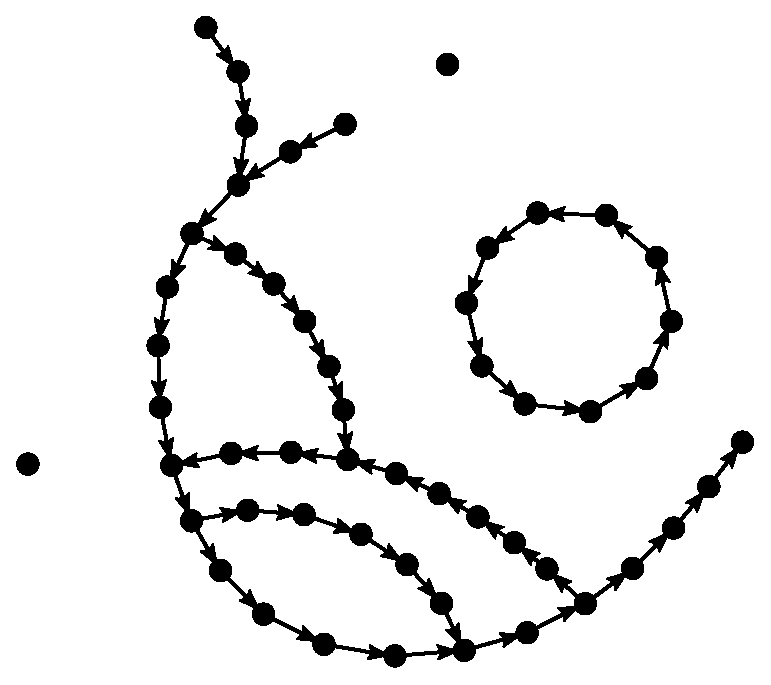
\includegraphics[width=0.90\textwidth]{Content/Pictures/kernel1.eps}
        \caption{$\vec{G}$}
    \end{subfigure}
    \hfill
    \begin{subfigure}[htbp]{0.45\textwidth}
        \centering
        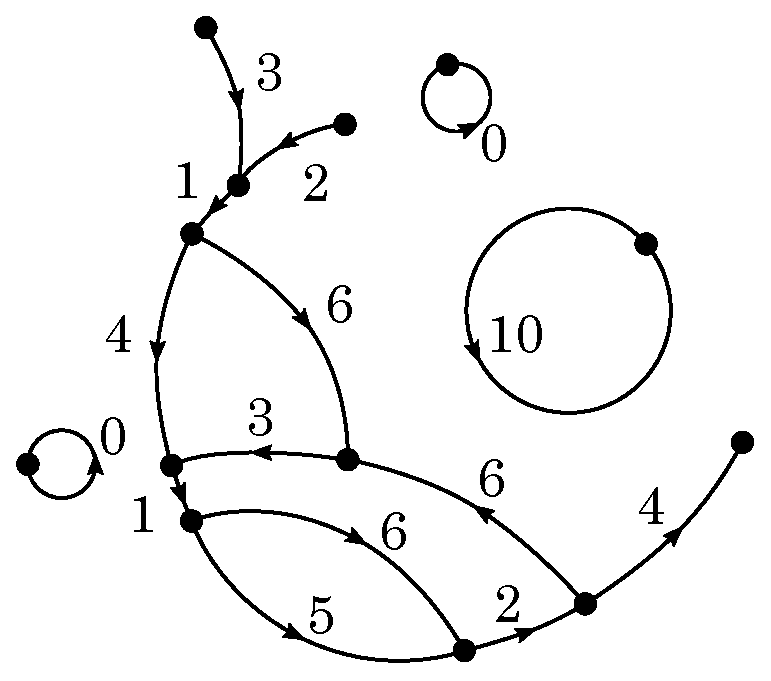
\includegraphics[width=0.90\textwidth]{Content/Pictures/kernel2.eps}
        \caption{$\kernel(\vec{G})$}
    \end{subfigure}
    \caption{An example of a digraph $\vec{G}$ and its kernel $\kernel(\vec{G})$}
    \label{fig:kernel}
\end{figure}

Consider an MDM $M$ and a vertex $w \in M$ with in-degree 1 and out-degree 1 which is not a self-loop. Let $u$ and $v$ be the unique in-neighbour and out-neighbour of $w$ respectively. The MDM obtained by smoothing $w$ is obtained by deleting the edges $e_1$ and $e_2$ such that $r(e_1) = (u, w)$ and $r(e_2) = (w, v)$, then adding an edge $e$ such that $r(e) = (u, v)$ and assigning it length $l(e) = l(e_1) + l(e_2)$. This is illustrated in \cref{fig:smoothing}. Then the kernel of a digraph $\vec{G}$ is obtained by doing the following:
\begin{enumerate}
    \item Assign a length $1$ to each edge.
    \item Iteratively smooth vertices with in-degree 1 and out-degree 1 that are not self-loops until there are none remaining.
    \item Replace all singletons by $\zeroloop$.
\end{enumerate}
Denote the resulting MMD by $\kernel(\vec{G})$. An example is shown in \cref{fig:kernel}.

\subsection{Our results}

Our main result is as follows. Let $C_i(n)$ for $i\geq 1$ be the kernels of the strongly connected components of $\vec{G}_n(\nu)$, listed in decreasing order of size, breaking ties arbitrarily. Complete the list with an infinite repeat of $\zeroloop$. Then, the main theorem is as follows.
\begin{theorem}\label{thm.main}
There exists a sequence $\cC=(\cC_i,i\in \N)$ of random strongly connected MDMs such that, for each $i\geq 1$, $\cC_i$ is either $3$-regular or a loop, and such that 
$$\left(n^{-1/3}C_i(n),i\in \N\right)\overset{d}{\to}\left(\cC_i,i\in \N\right)$$
as $n\to \infty$, with respect to the product $d_{\vec{\cG}}$-topology. The scaling is on lengths in the MDMs.
\end{theorem}
We see here why it is important to consider singletons as loops of length zero. For any fixed $k$, the $k$th largest SCC will not be a singleton with high probability. Therefore no component of our limiting object will be a singleton. Thus we need to pad our SCCs by $\zeroloop$ and consider the kernel of singletons to be $\zeroloop$ so that distance to the limiting object remains finite.

The law of the limit object places our model in the universality class of the directed Erd\H{o}s-Rényi model as studied by \citet{goldschmidtScalingLimitCritical2019}. This is the content of the following Corollary.
\begin{corollary}
Consider $\vec{G}_n(\nu)$, with $\nu$ such that $$\sigma_+=1=\frac{\sigma_{-+}+\nu_-}{\mu}=\frac{\sigma_{-+}+\nu_-}{\mu^2}=1.$$ (Note that this condition is satisfied by $\nu(k^-,k^+)=\nu_1(k^-)\nu_2(k^+)$, with $\nu_i$ the law of a $\operatorname{Poisson}(1)$ random variable.)
Let $(C_i(n), i\geq 1)$ be the strongly connected components of $\vec{G}_n(\nu)$, such that by Theorem \ref{thm.main} there exists $\cC=(\cC_i,i\in \N)$ such that 
$$\left(n^{-1/3}C_i(n),i\in \N\right)\overset{d}{\to}\left(\cC_i,i\in \N\right)$$
as $n\to \infty$, with respect to the product $d_{\vec{\cG}}$-topology. Also consider the directed Erd\H{o}s-R\'enyi model on $n$ vertices, in which any directed edge is present independently with probability $1/n$, which we denote by $\vec{G}(n,1/n)$, and let $(C'_i(n), i\geq 1)$ be the strongly connected components of $\vec{G}_n(\nu)$. Then, also
$$\left(n^{-1/3}C'_i(n),i\in \N\right)\overset{d}{\to}\left(\cC_i,i\in \N\right)$$
as $n\to \infty$, with respect to the product $d_{\vec{\cG}}$-topology. 
\end{corollary}
Moreover, Theorem \ref{thm.main} has the following trivial corollaries, which were previously unknown. 
\begin{corollary}
There exists a random sequence $(\ell_i,i\in \N)\in \R_+^\infty$, such that for $(L^n_i,i\in \N)$ the total lengths in the strongly connected components of $\vec{G}_n(\nu)$ ordered by decreasing length (appended with an infinite repeat of $0$), and for $(S^n_i,i\in\N)$ the number of vertices in the the strongly connected components of $\vec{G}_n(\nu)$ ordered by decreasing size (appended with an infinite repeat of $0$),
$$\left(n^{-1/3}L^n_i,n^{-1/3}S^n_i, i\in \N\right)\overset{d}{\to}\left(\ell_i,\ell_i,i\in \N\right)$$
as $n\to \infty$ in the product topology on $(\R^2)^\infty$. 
\end{corollary}
\begin{corollary}
For $v,w\in \vec{G}_n(\nu)$ such that $v\to w$, let $d(v,w)$ denote the length of the shortest path from $v$ to $w$, and let $$\operatorname{Diam}\left(\vec{G}_n(\nu)\right)=\max\{d(v,w):v\to w\}$$ be the \emph{diameter} of $\vec{G}_n(\nu)$. Then,  $$\operatorname{Diam}\left(\vec{G}_n(\nu)\right)=\Omega(n^{1/3})$$
with high probability.
\end{corollary}


\subsection{Previous work}
The configuration model was introduced by \citet{Bollobas1980} to sample a uniformly random graph with a given degree sequence. For a discussion of the configuration model and proofs of standard results, we refer the reader to \cite[Chapter 7]{hofstadRandomGraphsComplex2017}.

Most results on the configuration model are obtained for models with a deterministic degree sequence. The phase transition for undirected setting was shown in \cite{molloyCriticalPointRandom1995, Molloy1998, Janson2009}. The law of component sizes at criticality and in the critical window were obtained by \citet{Riordan2012} under the assumption that the degrees are bounded. Dhara, van der Hofstad, van Leeuwaarden and Sen showed convergence of the size and surplus edges in the critical window in the finite 3rd moment setting \cite{Dhara2017} and in the heavy-tailed regime \cite{Dhara2020}.  Bhamadi, Dhara, van der Hofstad and Sen obtained metric space convergence in the critical window in \cite{Bhamidi2020}, a result that the authors later improved to a stronger topology in \cite{Bhamidi2020Glmb}. 

Configuration models with a random degree sequence are considered in \cite{josephComponentSizesCritical2014}, \cite{conchon--kerjanStableGraphMetric2020}, and \cite{Donderwinkel2021heightprocess}. \citet{josephComponentSizesCritical2014} showed convergence of the component sizes and surpluses of the large components under rescaling at criticality, both for degree distributions with finite third moments and for the heavy-tailed regime. \citet{conchon--kerjanStableGraphMetric2020} show Gromov-Hausdorff-Prokhorov convergence at criticality in these two regimes. The results in \cite{conchon--kerjanStableGraphMetric2020} in the heavy-tailed regime are extended to the critical window by \citet{Donderwinkel2021heightprocess}. Our techniques are closely related to the techniques introduced in \cite{conchon--kerjanStableGraphMetric2020}. 

Some results have been obtained for other directed graph models. \citet{caoConnectivityGeneralClass2019} consider a class of inhomogeneous directed graphs. Their results include a phase transition for the existence of a giant strongly connected component. This is a generalisation work by \citet{Bloznelis2012}, in which a smaller class of inhomogeneous directed graphs is considered. \citet{Samorodnitsky2016} studied the tails of the degree distribution in the directed preferential attachment model. \citet{goldschmidtScalingLimitCritical2019} studied the directed Erd\H{o}s-R\'enyi model, and were the first to obtain metric space convergence of the strongly connected components of a directed graph. Our methods build on their techniques.

The directed configuration model was first considered by \citet{cooperSizeLargestStrongly2004}. They consider a deterministic degree sequence under a number of conditions, and show that for $\theta$ the expected in-degree of a uniformly chosen vertex, and $\rho$ the expected product of in-degree and out-degree of a uniformly chosen vertex, a phase transition for the strongly connected components occurs at $d=\theta/\rho=1$. They show that for $d<1$, with high probability, all strongly connected components contain $O(\Delta\log(n))$ vertices, for $\Delta$ the maximal degree. On the other hand, for $d>1$, there is a unique strongly connected components that contains a positive proportion of the vertices and also $O(n)$ edges. Their conditions are restrictive, and include finite second moments of both the in- and out-degree of a uniformly chosen vertex, and a bound of size $n^{1/12}/\log(n)$ on the largest degree. Their proofs are based on an algorithm to explore the directed graph. The condition on the largest degree was later relaxed to $O(n^{1/4})$ by \citet{Graf2016}.\myworries{check this is the phase transition}

Recently, Cai and Perarnau have obtained a number of results on the directed configuration model with deterministic degrees. In \cite{caiDiameterDirectedConfiguration2020}, they show, under first and second moment conditions of the degree of a uniformly picked vertex, for $d\neq 1$ (i.e. not at criticality), that the diameter of the model on $n$ vertices, rescaled by $\log(n)$ converges to a constant that they identify. Then, in \cite{caiGiantComponentDirected2020}, they show a law of large numbers for the number of vertices and edges in the largest strongly connected component, under slightly stronger moment conditions, and again not at the critical point. In \cite{cai2021rw}, they study the behaviour of a random walk on a directed configuration model.
 
The emergence of a giant weakly connected component for the directed configuration model with a deterministic degree sequence is discussed in the physics literature by \citet{Kryven2016}. He also studies the distribution of the in- and out-components in \cite{Kryven2017}.

The directed configuration model with random in- and out-degrees is also considered by \citet{Chen2012}, although, importantly, they do not allow for the in- and out-degree of a vertex to be dependent. The authors consider a model in which the in- and out-degrees are two independent sequences of i.i.d.\ random variables drawn from two probability distributions. They propose an algorithm to sample degree sequences that correspond to a simple graph and show the limiting distribution of the degrees generated by this algorithm. 


\subsection{Proof outline}

The techniques we will use to investigate the graph model are a combination of the techniques introduced by Conchon-Kerjan and Goldschmidt in \cite{conchon--kerjanStableGraphMetric2020} and the strategy of Goldschmidt and Stephenson in \cite{goldschmidtScalingLimitCritical2019}. The former work discusses the scaling limit of an undirected uniform graph with i.i.d.\ degrees at criticality, and the latter discusses the scaling limit of the strongly connected components of a directed Erd\H{o}s-Renyi graph at criticality.

To investigate the structure of the strongly connected components of a uniform graph with degree sequence $(\mathbf{D}_1,\dots,\mathbf{D}_n)$, conditional on $\sum_{i=1}^n D^-_i=\sum_{i=1}^n D^+_i$, we will use a version of the configuration model for digraphs that was introduced by \citet{cooperSizeLargestStrongly2004}.

Consider a degree sequence $\vd_1, \ldots, \vd_n$ where $\vd_i = (d_i^-, d_i^+) \in \N \times \N$. We assume 
\begin{equation*}
    \textstyle\sum_{i=1}^n d_i^- = \sum_{i=1}^n d_i^+. 
\end{equation*}
To sample the \emph{directed configuration model} with degree sequence $\vd_1, \ldots, \vd_n$ let $v_1, \ldots, v_n$ be vertices such that $v_i$ has $d_i^-$ in-half-edges and $d_i^+$ out-half-edges. We then pair the in-half-edges and out-half-edges uniformly. This results in a random directed multigraph. The directed configuration model is obtained by This is illustrated in Figure \ref{fig.configuration model}. 

If we then condition on the multigraph being simple, we would get a uniform random digraph on $[n]$ conditioned to have the given degree sequence. This is shown by \citet[P. 10--11]{cooperSizeLargestStrongly2004}. 

To explore the structure of a directed multigraph, we describe an edge-based depth first search procedure (eDFS) in \cref{alg:edfs}. This takes as input a directed multigraph and uses a stack of edges. When the stack is empty, we are at the start of a new out-component and thus pick a new vertex $w$ with probability proportional to its in-degree (this choice simplifies \myworries{insert lemma}). Otherwise we remove the last edge $(v, w)$ off the stack. In both cases, if $w$ has not yet been explored, we add the out-edges from this vertex to the end of the stack of edges (this choice is what makes the exploration depth first).

\myworries{define surplus edges and ordering of vertices}

At each step we also maintain $S^-(k)$ and $S^+(k)$. $S^-(k)$ keeps track of the number of in-edges which we have seen but have not explored the tail of yet at step $k$. $S^+(k)$ is akin to a Lukasiewiescz path. At any given step it is equal to the size of the stack of edges after subtracting the number of fully explored out-components.

We also construct a directed forest for which $S^-(k)$ will be a true Lukasiescz path. At each step of the process we will be examining a vertex $w$. If $w$ has not been explored yet then either we are at the start of a new out-component, in which case we add $w$ to the out-forest, or we are exploring an edge $(v, w)$ where $v$ has already been explored and added to the out-forest, in which case we add $w$ and the edge $(v, w)$ to the out-forest. If $w$ has already been explored we cannot add $(v, w)$ to the out-forest without creating loops. Instead add a dummy vertex to the out-forest and an edge from $v$ to the dummy vertex. We call such dummy vertices purple leafs. This is illustrated in Figure \ref{fig.configuration modeloutforest}. We refer to the out-forest corresponding to the exploration up to time $k$ as $\hat{F}_n(k)$.

\def \exploredvertices {\mathcal V}
\def \explorededges {\mathcal E}
\def \forest {\mathcal F}
\def \edgestack {\mathcal O}
\begin{algorithm}[htbp]
    \SetAlgoLined
    \KwData{A directed multigraph}
    $\exploredvertices \leftarrow$ an empty ordered list of vertices\;
    $\edgestack \leftarrow$ an empty ordered list of edges\;

    $k \leftarrow 0$ \;
    $S^- \leftarrow 0$ \;
    $S^+ \leftarrow 0$ \;
    $\forest \leftarrow$ an empty directed graph\;
    \While(){there exists unexplored vertices of positive in-degree}{
        \eIf(){$\edgestack$ is empty}{
            $w \leftarrow$ a random vertex not in $\exploredvertices$ chosen with prob.\ proportional to $d^-(w)$ \;
        }(){
            $e \leftarrow$ last edge in $\edgestack$ \;
            remove $e$ from $\edgestack$ \;
            $v \leftarrow$ tail of $e$\;
            $w \leftarrow$ head of $e$ \;
            $S^- \leftarrow S^- - 1$ \;
        }
        \eIf(){$w \not \in \exploredvertices$}{
            append $w$ to $\exploredvertices$ \; 
            add the vertex $w$ to $forest$ \;
            \If(){$\edgestack$ is non-empty}{
                add the edge $(v, w)$ to $\forest$\;
            }
            append all out-edges of $w$ to the end of $\edgestack$ in a uniform random order \;
            $S^- \leftarrow S^- + d^-(w)$ \;
            $S^+ \leftarrow S^+ + d^+(w) - 1$ \;
        }{
            add a purple leaf to $\forest$ and and edge from $v$ to the leaf \;
        }
        $k \leftarrow k + 1$ \;
        $S^-_k \leftarrow S^-$ \;
        $S^+_k \leftarrow S^+$ \;
        $\forest_k \leftarrow \forest$ \;
    }
    \caption{The eDFS procedure \label{alg:edfs}}
\end{algorithm}

\begin{figure}
    \centering
    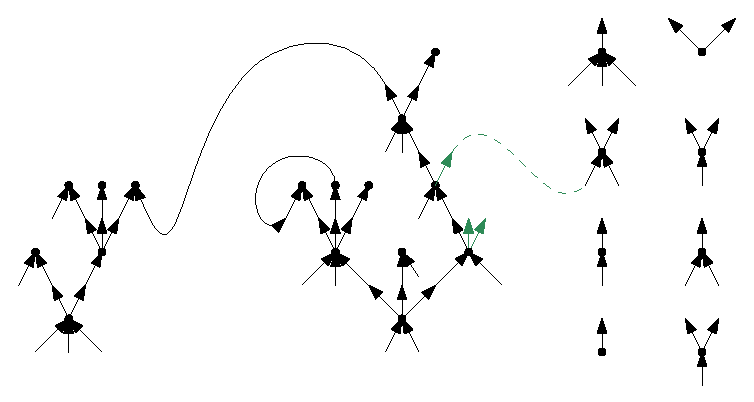
\includegraphics[scale=0.6]{Content/Pictures/configuration_model.eps}
    \caption{The green arrows represent unpaired out-half-edges of vertices that have been visited. One by one, in depth first order, these are paired to a uniform unpaired in-half-edge.}
    \label{fig.configuration model}
\end{figure}

An important motivation for studying the out-forest is the fact that the vertex set of any strongly connected component is contained in one of the components of the out-forest. This is a straightforward property that is further discussed in Lemma \ref{lemma.whatispartofscc}. We have defined the out-forest in such a way that every time step in the exploration corresponds to one vertex in the out-forest. 

A key fact is that the order in which the vertices are discovered does not depend on the position of the purple vertices. Similarly, the position of the purple vertices does not depend on the position of the heads of the surplus edges. Furthermore, we define a necessary condition for a surplus edge to be part of a strongly connected component (see Definition \ref{def.candidate} and Corollary \ref{cor.edgesinSCCs}), and we call these surplus edges \emph{candidates}. The candidates are defined in such a way that whether a purple vertex is a candidate does not depend on the position of the heads of the surplus edges. This allows us to define the following sampling procedure.
\begin{enumerate}
    \item We sample the order of discovery of the vertices in the exploration.
    \item We sample at which time steps a surplus edge is added instead of an edge to an undiscovered vertex, which allows us to define the out-forest $(\hat{F}_n(k),k\geq 1)$. 
    \item We visit the purple vertices in $(\hat{F}_n(k),k\geq 1)$ in depth-first order, and for each vertex we sample whether it corresponds to a candidate.
    \item We visit the tails of the candidates in depth-first order, and for each of them, sample where the head of the corresponding surplus edge is.
\end{enumerate}

\begin{figure}
    \centering
    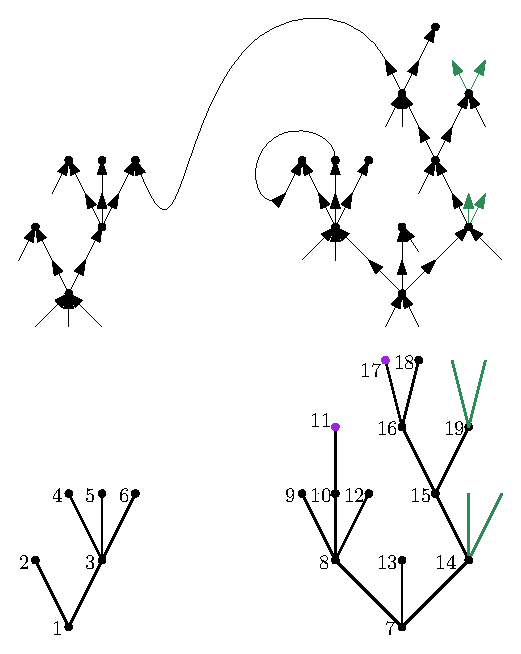
\includegraphics[scale=0.8]{Content/Pictures/configuration_model_out_forest.eps}
    \caption{The out-forest is defined based on the exploration of the digraph. For each surplus edge, we add an extra leaf, which we colour purple. The labels of the vertices correspond to the time step in the exploration at which the vertex is added. The green edges lead to vertices of which the degree and colour have not yet been sampled.}
    \label{fig.configuration modeloutforest}
\end{figure}
Then, our approach is as follows.
\begin{enumerate}
    \item We find the limit under rescaling of the \L ukasiewicz path and height process of $\hat{F}_n(m_n)$ for $m_n=O(n^{2/3})$ conditional on $\sum_{i=1}^n D^-_i=\sum_{i=1}^n D^+_i$ and simplicity of the digraph. (For a definition of the \L ukasiewicz path and height forest, see \cite{AST_2002__281__R1_0}, Chapter 0.)
    \item We show that the positions of the tails of the candidates converge.
    \item We show that the positions of the heads of the candidates converge.
    \item We identify the tails and heads of the candidates, and recover the strongly connected components from the resulting digraph with a cutting procedure. We use a result in \cite{goldschmidtScalingLimitCritical2019} that implies that the cutting procedure converges.
    \item We show that for any $\delta>0$, with high probability, all strongly connected components with length larger than $\delta n^{1/3}$ are contained in the exploration up to time $O(n^{2/3})$. Therefore, we can choose $m_n$ such that, with high probability, we do not miss any large strongly connected components by not considering the exploration beyond time $m_n$. This finishes the proof of the convergence in the product topology.
\end{enumerate}

\subsection{Open problems}
Our work contains the first results on the directed configuration model at criticality, and is the second metric space convergence result for a directed graph model (after the directed Erd\H{o}s-Rényi graph was studied in \cite{goldschmidtScalingLimitCritical2019}), so naturally, there are many interesting unresolved questions.
\begin{enumerate}
    \item The law of our limit object is defined by three parameters that are functions of the (mixed) moments of the degree distribution. Does a different choice of parameters always give a different limit distribution? If so, are the laws absolutely continuous to one another?
    \item Our methods show that the diameter of the configuration model at criticality is  $\Omega(n^{1/3})$, which is in contrast with the off-critical cases (for deterministic degrees), in which the diameter is $O(\log(n))$ \cite{caiDiameterDirectedConfiguration2020}. We believe that the diameter is in fact exactly $O(n^{1/3})$. Goldschmidt and Maazoun are working on this question for the directed Erd\H{o}s-Rényi graph at criticality. 
    \item In \cite{goldschmidtScalingLimitCritical2019}, the authors show convergence of the sequence of SCCs in the $\ell_1$-sense, which is stronger than the product topology as considered by us. This for example implies that for the directed Erd\H{o}s-Rényi graph, the total length in the SCCs converges in distribution to some finite number. Also for undirected configuration models, there are no results that show metric space convergence in a topology on the sequence of components that is stronger than the product topology \cite{Bhamidi2020}\cite{conchon--kerjanStableGraphMetric2020}\cite{Bhamidi2020Glmb}.
     \item We conjecture that, just like the directed Erd\H{o}s-Rényi graph \cite{goldschmidtScalingLimitCritical2019}, the directed configuration model gives rise to a critical window, that in some sense interpolates between subcritical and supercritical models. It would be interesting to adapt our methods to the critical window.
     \item We plan to extend our understanding of the strongly connected components by studying the directed graphs that they are embedded in. A first step would be to study all vertices that can be reached from the non-trivial strongly components. This would illuminate connections between the strongly connected components and expose the fractal structure of the directed graph, which is not observed when only studying the strongly connected components themselves.
    \item Another natural next step is to study the model under weaker moment conditions. The first condition to eliminate is $\E\left[(D^-)^i(D^+)^j\right]$ for $\{i,j\}=\{1,3\}$, which would in some sense makes the identifications less uniform on the ancestral lines. We have reason to believe that this would place the model in  a different universality class, but further research is needed to confirm this. Also the heavy-tailed case is not well-understood, but given our results, it is natural to expect the limit object to be embedded in a tilted stable tree as defined in \cite{conchon--kerjanStableGraphMetric2020}. Moreover, one could define hybrid models by letting the tail-behaviour of the in- and out-degrees be different. 
    \item We conjecture that the inhomogeneous directed random graph model under suitable conditions is part of the same universality class as the directed Erd\H{o}s-Rényi graph \cite{goldschmidtScalingLimitCritical2019} and $\vec{G}_n(\nu)$. We believe that our methods and the methods of \cite{goldschmidtScalingLimitCritical2019} can be adapted to obtain a metric space scaling limit for the inhomogeneous directed random graph model. 

\end{enumerate}


\section{Sampling the MDM in the discrete and the continuum}
If we forget about the directions of the edges, the graph is supercritical, and the graph contains a unique giant component with surplus going to infinity as $n\to \infty$. This suggests that if we do not dismiss a large amount of edges, we will not be able to study the digraph in enough detail to find a metric space scaling limit of the strongly connected components. Therefore, we will not try to sample the entire digraph, but focus on the information that we need to find the strongly connected components. We start by studying the discrete graph model, with the goal of identifying which edges can be part of a strongly connected components, and how to sample them. In Subsubsection \ref{subsubsec.defcandidates}, we establish necessary conditions for an edge to be part of a strongly connected component. The result implies that we only need to study the out-forest, and a small subset of the surplus edges, which we call \emph{candidates}. In Subsubsections \ref{subsubsec.samplingoutforest} and \ref{subsubsec.samplecandidates} we study the law of the out-forest and the candidates respectively, and we define a procedure to sample both. This yields a sequence of directed multigraphs with edge lengths that the strongly connected components are embedded in.  
In Subsection \ref{subsec.limitobject}, we define the continuous counterpart of the sampling procedure. The resulting object will the limit under rescaling of the sequence of directed multigraphs with edge lengths that the strongly connected components are embedded in that was constructed in Subsubsections \ref{subsubsec.samplingoutforest} and \ref{subsubsec.samplecandidates}. 
\subsection{The discrete case}\label{subsec.discrete}
We will discuss the different type of edges that we can encounter in the exploration. By slight abuse of notation, we call the purple vertex that corresponds to a surplus edge its tail.

\subsubsection{Necessary conditions for an edge to be part of an SCC}\label{subsubsec.defcandidates}
Amongst the surplus edges, \emph{ancestral surplus edges}, which are surplus edges that point from a vertex to one of its ancestors, play a special rôle. All other surplus edges are called non-ancestral. This is illustrated in Figure \ref{subfigure.typesofsurplusedges}. In Figure \ref{subfigure.sccinexample} we show how surplus edges affect the structure of the strongly connected components. This is the content of Lemma \ref{lemma.whatispartofscc}.
\begin{lemma}\label{lemma.whatispartofscc}
The following facts hold for strongly connected components. 
\begin{enumerate}
\item \label{item.factsonsccs1}The vertices of a strongly component are contained in one of the components of $(\hat{F}_n(k),k\geq 1)$. 
\item \label{item.factsonsccs2} Ancestral surplus edges are always part of a strongly connected component.
\item \label{item.factsonsccs4} A non-ancestral surplus edge is only part of a strongly connected component if its head is an ancestor of the tail of a surplus edge that is part of a strongly connected component.
\item \label{item.factsonsccs4andabit} An edge in $(\hat{F}_n(k),k\geq 1)$ is only part of a strongly connected component if its head is an ancestor of the tail of a a surplus edge that is part of a strongly connected component.
\item \label{item.factsonsccs5} For any non-trivial strongly connected component, the first surplus edge of the SCC that is explored is an ancestral surplus edge, and a component of  $(\hat{F}_n(k),k\geq 1)$ contains a strongly connected component if and only if it contains an ancestral surplus edge.
\end{enumerate}
\end{lemma}
\begin{proof}
We start with \ref{item.factsonsccs1}. Let $v$ and $w$ be two vertices in the same strongly connected component. Without loss of generality, $v$ is explored first in depth-first order in the out-direction. Since $v$ and $w$ are part of the same strongly connected component, we know that there is a path from $v$ to $w$ in the out-direction. This implies that $w$ will be part of the out-subtree rooted at $v$. This implies that they are part of the same component of $(\hat{F}_n(k),k\geq 1)$. \\
To prove \ref{item.factsonsccs2}, suppose there is an ancestral surplus edge from $v$ to $w$. This implies that $w$ is an ancestor of $v$ in an out-component, which implies that there is a path from $w$ to $v$ as well. It follows that $w$ and $v$ are in the same strongly connected component and that the ancestral surplus edge from $v$ to $w$ is in this strongly connected component as well. \\
To prove \ref{item.factsonsccs4}, suppose we sample a non-ancestral surplus edge from $v$ to $w$ that is part of a strongly connected component. Then, by \ref{item.factsonsccs2}, there is a path from $w$ to $v$ present at the time of sampling $(v,w)$. Let $(x,y)$ be the first surplus edge on this path. This implies that $(x,y)$ is in the same strongly connected component as $v$ and $w$. Moreover, the path from $w$ to $x$ consists of edges in the out-forest, $x$ is a descendant of $w$.\\
Next, for \ref{item.factsonsccs4andabit}, suppose $(v,w)$ is an edge of $(\hat{F}_n(k),k\geq 1)$ that is part of a strongly connected component. This means that there is a path from $w$ to $v$. Let $(x,y)$ be the first edge on this path such that $y$ is not a descendant of $w$. Then, $(x,y)$ is a surplus edge that is part of the same strongly connected component as $v$ and $w$, and $(v,w)$ is on the path from the root to $x$. \\
Finally, \ref{item.factsonsccs2} and \ref{item.factsonsccs4} imply \ref{item.factsonsccs5}. 
\end{proof}

Lemma \ref{lemma.whatispartofscc} motivates the following definition.
\begin{definition}\label{def.candidate}
A surplus edge is a \emph{candidate} if either
\begin{itemize}
    \item It is an ancestral surplus edge, or
    \item One of the descendants of its head is the tail of a candidate.
\end{itemize}
\end{definition}
The following corollary is at the core of our strategy to study the strongly connected components.
\begin{corollary}\label{cor.edgesinSCCs}
All edges that are part of a strongly connected component are either a candidate, or are contained in the subforest of $(\hat{F}_n(k),k\geq 1)$ that is spanned by the tails of candidates and the component roots.
\end{corollary}
\begin{proof}
This follows from Definition \ref{def.candidate} and parts \ref{item.factsonsccs1}, \ref{cond.excursions2}, \ref{item.factsonsccs4} and \ref{item.factsonsccs5} of Lemma \ref{lemma.whatispartofscc}.
\end{proof}
\begin{figure}
\centering
\begin{subfigure}{0.7\textwidth}
 \centering
    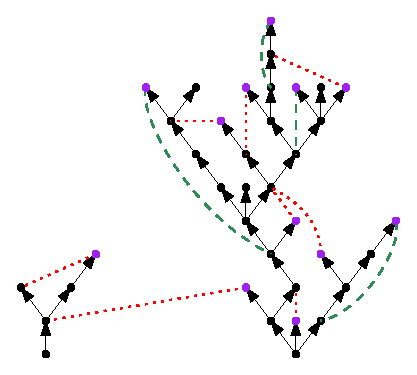
\includegraphics[width=0.7\linewidth]{Content/Pictures/types_of_surplus_edges.eps}
    \caption{This figure illustrates an example of a depth-first exploration of two out-components with the different type of surplus edges highlighted. The ancestral surplus edges (green dashed) point from a vertex $v$ to one of its ancestors. They are always part of a strongly connected component. The other surplus edges are depicted as red dotted lines.}
    \label{subfigure.typesofsurplusedges} 
\end{subfigure}\\
\begin{subfigure}{0.7\textwidth}
  \centering
  \includegraphics[width=0.7\linewidth]{Content/Pictures/sccs_in_example.eps}
  \caption{The non-trivial strongly connected components embedded in the components of the out-forest are depicted in orange, blue and green. The trivial strongly connected components are black. The grey edges are not part of a strongly connected component, and the grey vertices correspond to purple leaves that are not part of a strongly connected component.}
    \label{subfigure.sccinexample}
\end{subfigure}
\caption{We illustrate the different types of surplus edges and how they affect the structure of the strongly connected components.}
\end{figure}

Corollary \ref{cor.edgesinSCCs} implies that for every purple vertex, we only need to know whether it is a candidate, and if so, where its head is. 
\subsubsection{Sampling the out-forest}\label{subsubsec.samplingoutforest}
This subsubsection discusses how to obtain the out-forest conditional on the order in which the vertices are discovered. We will study the law of the degrees in order of discovery in Subsection \ref{subsec.measurechange}. Informally, the out-forest is obtained in the following way. Suppose the degrees in order of discovery are given by $(\mathbf{\hat{D}}_{n,1},\dots,\mathbf{\hat{D}}_{n,n})$. Up to time step $k$, suppose we have added the vertices corresponding to the first $m\leq k$ elements of  $(\mathbf{\hat{D}}_{n,1},\dots,\mathbf{\hat{D}}_{n,n})$ to the forest. We call these vertices \emph{discovered}. Then, at time $k+1$,
\begin{enumerate}
    \item If we have finished a component of the out-forest, let the next component have a root with out-degree $\hat{D}_{n,m+1}^+$. 
    \item Otherwise,
    \begin{enumerate}\item With probability proportional to the total in-degree of the undiscovered vertices, i.e. $\sum_{i={m+1}}^n \hat{D}_{n,i}^-$, let the next vertex in depth-first order be a black vertex with out-degree $\hat{D}_{n,m+1}^+$.
    \item With probability proportional to the unpaired in-half-edges of the $l$ discovered vertices, let the next vertex in depth-first order be a purple leaf, and reduce the number of unpaired in-edges of the $l$ discovered vertices by $1$.
\end{enumerate}
\end{enumerate}
We make this rigourous in the following lemma.
\begin{lemma}\label{lemma.sampleoutforest}
Suppose the sequence of degrees in order of discovery $(\hat{D}^n_1,\dots,\hat{D}^n_n)$ is given. Suppose, for $1\leq l\leq k$, that up to time $l$, $\hat{P}_n(l)$ surplus edges have been sampled. Then, $$\left(\hat{S}^+_n(l),1\leq l\leq k \right):=\left(\sum_{i=1}^{l-\hat{P}_n(l)}\hat{D}^+_{n,i}-l,1\leq l\leq k\right)$$ is the \L ukasiewicz path of the out-forest up to time $k$. Moreover, for $$\left(\hat{I}^+_n(l),1\leq l\leq k\right):=\left(\min\left\{\hat{S}^+_n(m):1\leq m \leq l\right\},1\leq l \leq k \right),$$
define 
$$\left(\hat{S}^-_n(l),1\leq l \leq k\right):=\left(\sum_{i=1}^{l-\hat{P}_n(l)}\hat{D}^-_{n,i}-l-\hat{I}^+_n(l)+1,1\leq l\leq k\right),$$
so that $\hat{S}^-_n(k)$ is equal to the number of unpaired in-half-edges of discovered vertices at time $k$. Then, the probability that we sample a surplus edge at the $(k+1)^{th}$ time step is given by
$$\frac{\hat{S}^-_n(k+1)}{\sum_{i=1}^n D^-_i-k-\hat{I}^+_n(k)+1}\one_{\left\{\hat{I}^+_n(k)=\hat{I}^+_n(k-1)\right\}}.$$
Therefore, we do not need to know the position of the heads of the surplus edges to sample the out-forest.
\end{lemma}
\begin{proof}
Note that if up to time $k$, $\hat{P}_n(k)$ surplus edges have been sampled, this implies that $k-\hat{P}_n(k)$ vertices have been discovered. Thus, up to time $k$, the out-forest contains $\hat{P}_n(k)$ purple leaves, and black vertices with degrees $(\hat{D}^+_{n,1},\dots,\hat{D}^+_{n,k-\hat{P}_n(k)})$, so by definition of the \L ukasiewicz path, its value is indeed equal to $\hat{S}^-_n(k)$ at time $k$. Moreover, up to time $k$, the total in-degree of discovered vertices is equal to $\sum_{i=1}^{k-\hat{P}_n(k)}\hat{D}^-_{n,i}$. At every time step, we pair $1$ in-half-edge of a discovered vertex, unless we start a new component. $-\hat{I}^+_n(k)$ corresponds to the number of out-components that are finished up to time $k$, so the total number of unpaired in-half-edges of discovered vertices at time $k$ is equal to $\hat{S}^-_n(k)$. By the same reasoning, the total number of unpaired in-half-edges is equal to $\sum_{i=1}^n D^-_i-k-\hat{I}^+_n(k)+1$. The probability of sampling a surplus edge follows. We note that this probability does not depend on the position of the heads of the surplus edges, which implies that we can sample the out-forest without this information.
\end{proof}
\subsubsection{Sampling the candidates}\label{subsubsec.samplecandidates}
We will now study the law of the candidates conditional on $(\hat{F}_n(k),k\geq 1)$. As before, for each $k$, let $\hat{P}_n(k)$ denote the number of purple vertices amongst the first $k$ vertices in the out-forest, and let $\hat{S}^-(k)$ denote the number of unpaired in-half-edges of discovered vertices at time $k$. We will first identify the tails of the candidates amongst the purple vertices, and then we will sample the position of their heads. \\
If the vertex visited at time $k$ is purple, the head of the corresponding surplus edge is a uniform pick from the $\hat{S}^-(k)$ unpaired in-half-edges of discovered vertices at time $k$. Therefore, the probability that a purple vertex visited at time $k$ corresponds to an ancestral surplus edge is given by the number of unpaired in-edges on its path to the root divided by $\hat{S}^-(k)$. This implies that to understand the law of the position of ancestral surplus edges, we need to understand where the unpaired in-edges are. \\
We will study this by modifying the edge lengths in the tree: for a vertex $v$ with in-degree $m$, the edges connecting it to its children will have length $m-1$ (unless $v$ is the root of an out-component, then the edges connecting to its children will have length $m$). The height of vertex $w$ in this forest with edge lengths corresponds to the number of in-half-edges that can be used to form an ancestral surplus edge with tail $w$. We add lengths to all edges in $(\hat{F}_n(k),k\geq 1)$ and call the resulting forest with edge lengths $(\hat{F}^\ell(k),k\geq 1)$. Denote the height process of $(\hat{F}^\ell(k),k\geq 1)$ by $(\hat{H}_n^\ell(k),k\geq 1)$. \\
Recall that the first candidate in any component of $(\hat{F}_n(k),k\geq 1)$ is an ancestral surplus edge. The following lemma illustrates the importance of $\hat{H}^\ell$ in finding the first ancestral surplus edges in the out-components.

\begin{lemma}\label{lemma.probancestral}
Consider the exploration of $(\hat{F}_n(k),k\geq 1)$ at time $k$. If no ancestral surplus edge has been sampled in the current component, then the probability that $k$ is the tail of an ancestral surplus edge is given by 
$$a_k=\frac{\hat{H}^\ell(k)}{\hat{S}_n^-(k)}\one_{\{\hat{P}_n(k)-\hat{P}_n(k-1)=1\}}.$$
This event is independent of the position of the heads of the surplus edges that were found before time $k$.
% If $k$ is the tail of an ancestral surplus edge, then the position of the end point $Y$ has the following law. Let $U$ be uniform on $[0,\hat{H}^\ell(k)]$. Then, let $Y_k$ be the height of youngest ancestor $l$ of $k$ such that $H^{\ell}(l)<U$. 
\end{lemma}
\begin{proof}
We claim that if no ancestral surplus edge has been sampled in the current component, none of the ancestors of $k$ are the head of a surplus edge. Indeed, for $x$ an ancestor of $k$, all vertices that are visited since the discovery of $x$ up to time $k$ are descendants of $x$, because $(\hat{F}_n(k),k\geq 1)$ is explored in a depth-first manner. Therefore, any surplus edge with head $x$ sampled up to time $k$ is ancestral. This implies that for $d^-$ the in-degree of $x$, the number of unpaired in-half-edges of $x$ at time $k$ is equal to $d^--1$ (unless $x$ is the root of the out-component, in which case it has $d^-$ unpaired in-half-edges).

Therefore, the number of unpaired in-half-edges corresponding to ancestors of $k$ is equal to $H^\ell(k)$. Moreover, note that, by definition of the purple vertices, $k$ is the tail of a surplus edge if and only if $k$ is purple, i.e. if and only if $\hat{P}_n(k)-\hat{P}_n(k-1)=1$. In that case, the probability that it connects to given unpaired in-half-edge of a visited vertex is equal to $1/\hat{S}_n^-(k)$. The stated probability follows. The independence on the position of the heads of earlier surplus edges is immediate.
\end{proof}

We now illustrate how to find the other candidates in a component of $(\hat{F}_n(k),k\geq 1)$. 
\begin{lemma}\label{lemma.samplecandidates}
Let $T^n_{l_n}$ be a component of $(\hat{F}_n(k),k\geq 1)$ with root $l_n+1$ and component length $\sigma_n$. Suppose the first ancestral surplus edge in $T^n_{l_n}$ corresponds to purple vertex $V^n_1\in [l_n+2,l_n+\sigma_n]$. Let $V^n_1<k\leq l_n+\sigma_n$, and suppose the candidates found up to time $k$ are given by $V^n_1,\dots,V^n_m$. Let $T^{n,\text{mk}}_k$ be the subtree of $T^n_{l_n}$ spanned by $\{l_n+1,V^n_1,\dots,V^n_m,k\}$, and let $\ell(T^{n,\text{mk}}_k)$ be its total length with edge lengths as defined by $(\hat{H}^\ell(m),m\in [l_n+1,l_n+\sigma_n])$. Then, the probability that $k$ is a candidate is given by 
$$\frac{\ell\left(T^{n,\text{mk}}_k\right)-l}{\hat{S}^-(k)}\one_{\{\hat{P}_n(k)=\hat{P}_n(k-1)+1\}}.$$
\end{lemma}
\begin{proof}
Note that if $k$ is purple, it gets paired to a uniform pick from the $\hat{S}^-(k)$ unpaired in-half-edges of discovered vertices. By Definition \ref{def.candidate}, in that case, $k$ is a candidate if and only if its head is in $T^{n,\text{mk}}_k$. Observe that $\ell\left(T^{n,\text{mk}}_k\right)$ is equal to the number of in-half-edges of $T_{k}$ that can be used to form surplus edges. By the definition of a candidate, exactly $m$ of those have been paired: one for each element in $\{V^n_1,\dots,V^n_m\}$. This implies that $\ell\left(T^{n,\text{mk}}_k\right)-m$ of the $\hat{S}^-(k)$ options will cause $k$ to be a candidate.
\end{proof}

Note that the probability that a purple vertex corresponds to a candidate only depends on the out-forest and the number of candidates that have been found in the component so far. The position of the heads of the candidates can be found as follows.
\begin{lemma}\label{lemma.sampleheadcandidates}
Let $T^n_{l_n}$ be a component of $(\hat{F}_n(k),k\geq 1)$ with root $l_n+1$ and component length $\sigma_n$. Suppose its candidates are given by $\{V^n_1,\dots,V^n_{N_n}\}$. Then, for $1\leq i\leq {N_n}$, suppose the heads of the surplus edges corresponding to $V^n_1,\dots,V^n_{i-1}$ are given by $W_1^n,\dots,W^n_{i-1}$ respectively. Then, the in-half-edge that $V^n_{i}$ gets paired to is a uniform pick from the $$\ell\left(T^{n,\text{mk}}_{V^n_i}\right)-(i-1)$$ unpaired in-half-edges of $T^{n,\text{mk}}_{V^n_i}$ that remain. Call the corresponding vertex $W^n_i$.
\end{lemma}
\begin{proof}
Given that $V^n_{i}$ is a candidate, its head will be in $T^{n,\text{mk}}_{V^n_i}$. Then, the distribution follows.
\end{proof}

Lemmas \ref{lemma.sampleoutforest}, \ref{lemma.probancestral}, \ref{lemma.samplecandidates}, and \ref{lemma.sampleheadcandidates} justify the following sampling procedure.
\begin{enumerate}
    \item Sample the out-forest $(\hat{F}_n(k),k\geq 1)$.
    \item Fix $T>0$ and define a counting process $(A_n(k),k\leq \lfloor Tn^{2/3}\rfloor)$, with the probability of an increment at time $k$ given by $$a_k=\frac{\hat{H}_n^\ell(k)}{\hat{S}_n^-(k)}\one_{\{\hat{P}_n(k)-\hat{P}_n(k-1)=1\}}.$$
    \item For $i\geq 1$, set $X_i^n=\min\{k:A_n(k)=i\}$. Define
\begin{align*}L_i^n&=\min\left\{k\geq 1:\hat{S}^{+}_n(k)=\min\{\hat{S}^{+}_n(l):l\leq X_i^n\}\right\}\text{ for }i\geq 1\\
\Sigma_i^n&=\min\left\{k \geq 1: \min\left\{\hat{S}^{+}_n(l):l\leq L_i^n+k\right\} < \min\left\{\hat{S}^{+}_n(l):l\leq X_i^n\right\}\right\}\text{ for }i\geq 1,
\end{align*}
so that for each $i\geq 1$, $\left(\hat{S}^+(k),k\in [L_i^n+1,L_i^n+\Sigma_i^n]\right)$ encodes the tree containing $X_i^n$. For each $(l_n,\sigma_n)\in \{(L_i^n,\Sigma_i^n)\}$, let $T^n_{l_n}$ be the tree in $(\hat{F}_n(k),k\geq 1)$ with root $l_n+1$, and do the following.
    \begin{enumerate}
    \item \label{item.procedure3} Set $V_1^n=\min\{m\geq 1:A_n(m)=A_n(g)+1\}$, and find the other candidates $\{V_2^n,\dots ,V_{N_n}^n\}$ according to the procedure described in the statement of Lemma \ref{lemma.samplecandidates}.
    \item \label{item.procedure4} For $V_1^n,\dots, V_{N_n}^n$, sample their heads $W_1^n,\dots ,W_{N_n}^n$ respectively according to the procedure described in the statement of Lemma \ref{lemma.sampleheadcandidates}.
    \item Let $T^{n,\text{mk}}(l_n)$ be the subtree of $T^n_{l_n}$ spanned by $\{l_n+1,V_1^n,\dots ,V_{N_n}^n\}$, say $V_i^n\sim W_i^n$ for each $1\leq i\leq N_n$, and set $M^n_{l_n}:=T^{n,\text{mk}}_{l_n}/\sim$, which we note is a directed graph with surplus $N_n$. 
\end{enumerate}
\end{enumerate}
Then, all strongly connected components of $\vec{G}_n(\nu)$ of which the first candidate is sampled before time $\lfloor Tn^{2/3}\rfloor$ are subgraphs of $\left\{M^n_{L_i^n}, i\geq 1 \right\}$. Call these strongly connected components, ordered by decreasing size $(C_i^T(n),i\geq 1)$, completed with an infinite repeat of $\mathfrak{L}$. Observe that we may view $M^n_{L_i^n}$ as a finite rooted directed multigraph $M^n_{L_i^n}$ whose edges are endowed with lengths. To be precise, in  $M^n_{L_i^n}$, let the vertex set consist of $L_i^n+1$, $W_i^n$ for $i\leq N_n$, and the branch points $V_i^n\wedge V_j^n$ for $i\neq j\leq N_n$. Then, we obtain $(C_i^T(n),i\geq 1)$ by ordering the SCCs in $\left\{M^n_{L_i^n}, i\geq 1 \right\}$ by decreasing size, and completing the list with an infinite repeat of $\mathfrak{L}$. See Figure \myworries{picture Robin} for a sketch of this procedure.

\subsection{The continuum case}\label{subsec.limitobject}
We will define now define the continuous counterpart of the sampling procedure of the out-forest and the candidates. This is a slight modification of the procedure defined in Subsubsection 3.2.2 of \cite{Goldschmidt2019}. \\

\subsubsection{\texorpdfstring{$\R$}{R}-trees and their encoding}
The continuum analogue of discrete trees are given by $\R$-trees. A survey paper on $\R$-trees can be found in \cite{Legall2005}. An $\R$-tree is a compact metric space $(\cT, d)$ such that for every $a, b \in \cT$ the following two properties hold:
\begin{enumerate}
    \item There exists a unique isometry $i_{a, b} : [0, d(a, b)] \to \cT$ such that $i_{a, b}(0) = a$ and $i_{a, b}(d(a, b)) = b$.
    \item If $q: [0, 1] \to \cT$ is any continuous map such that $q(0) = a$ and $q(1) = b$ then the image of $q$ is the same as the image of $i_{a, b}$.
\end{enumerate}
Let $\pathbtw{a, b}$ denote the image of $i_{a, b}$. This is the unique path between $a$ and $b$.

$\R$-trees are often encoded by continuous excursions which can be seen as a continuous analogue of the height function of a tree. Let $f: [0, \sigma] \to [0, \infty)$ be a continuous excursion, meaning $f$ is continuous, $f(0) = f(\sigma) = 0$ and $f(x) > 0$ for all $x \in (0, \sigma)$. Using $f$ we can define a pseudo-metric
\begin{equation*}
    d_f(x, y) = f(x) + f(y) - 2 \min_{s \in [x \wedge y, x \vee y]} f(s).
\end{equation*}
Using this we can define the quotient space
\begin{equation*}
    \cT_f = [0, \sigma] / \{d_f = 0\}.
\end{equation*}
The space $\cT_f$ equipped with the metric $d_f$ is the $\R$-tree encoded by the excursion $f$. Let $p_f: [0, \sigma] \to \cT_f$ be the natural projection function. Then $\cT_f$ inherits a distinguished root vertex $\rho = p(0) = p(\sigma)$.

\subsubsection{The limit object}\label{subsubsec.samplecontinuousobject}
Let $(B_t,t\geq 0)$ be a Brownian motion, and set $$\left(\hat{B}_t,t\geq 0\right)=\left(B_t-\frac{\sigma_{-+}+\nu_-}{2\sigma_+\mu}t^2,t\geq 0\right).$$ 
\begin{remark}
We note that the coefficient of the parabolic drift is negative. Indeed, the sign of the parabolic drift is the same as the sign of $\mu-\E[D^+(D^-)^2]$, and we note that
$$\frac{\E[(D^-)^2D^+]}{\E[D^+]}-\left(\frac{\E[D^+D^-]}{\E[D^+]}\right)^2=\frac{\E[(Z^+)^2]}{\mu}-1$$
is the variance of $D^-$ under the law of $\mathbf{D}$ size-biased by $D^+$, which is positive. Hence $\E[D^+(D^-)^2]/\mu\geq 1$, which shows that $(\hat{B}_t)_{t\geq 0}$ is a Brownian motion with a downwards parabolic drift.
\end{remark}
Define 
$$(\hat{R}_t,t\geq 0)= \left(\hat{B}_t-\inf\left\{\hat{B}_s: s\leq t\right\},t\geq 0\right).$$
Then, it is standard that $\left(\frac{2}{\sigma_+}\hat{R}_t,t\geq 0\right)$ is the height process corresponding to an $\R$-forest with \L ukasiewicz path $\left(\sigma_+\hat{B}_t,t\geq 0\right)$.  This fact also follows from the argument in Section \ref{sec.convoutforest}. Call this forest $(\hat{\cF}(t),t\geq 0)$. \\
Let $(A_t,t\geq 0)$ be a Cox process of intensity $$\frac{2(\sigma_{-+}+\nu_-)}{\sigma_+\mu^2} \hat{R}_t$$ at time $t$. Then, fix $T>0$, so that $A_T<\infty$ almost surely. For $i$ in $\left[A_T\right]$, set $X_i=\min\{t:A_T=i\}$. Define
\begin{align*}
L_i&=\inf\left\{t\geq 0:=\hat{B}_t=\inf\{\hat{B}_s:s\leq X_i\}\right\}\text{ for }i\in \left[A_T\right]\text{ and}\\
\Sigma_i&=\inf\left\{ t\geq 0: \inf\{\hat{B}_s:s\leq L_i+t\} < \inf\{\hat{B}_s:s\leq X_i\}\right\}\text{ for }i\in \left[A_T\right],
\end{align*}
so that for each $i$ in $\left[A_T\right]$, $\left(\frac{2}{\sigma_+}\hat{R}_t,t\in [L_i,L_i+\Sigma_i]\right)$ encodes the $\R$-tree in $(\hat{\cF}(t),t\geq 0)$ that contains $X_i$. For each element of $\{(L_i,\Sigma_i):i\in A_T\}$ we will sample the candidates in the $\R$-tree. Fix $i$, and set $(l,\sigma)=[L_i,\Sigma_i]$. Let $V_1=\inf\{s>0:A(s)=A(l)+1\}$, so that $l\leq V_1\leq l+\sigma$ by definition of $(l,\sigma)$. Let $\cT_l$ be the $R$-tree encoded by $\left(\frac{2}{\sigma_+}\hat{R}_t,t\in [l,l+\sigma]\right)$ and let $p_l:[l,l+\sigma]\to \cT_l$ be the projection onto $\cT_l$ given by the encoding. Set $$||\cT_l||=\sup\left\{\frac{2}{\sigma_+}\hat{R}_t,t\in [l,l+\sigma]\right\},$$
which we note is the height of $\cT_l$. \\
Suppose we have found candidates $\{V_1,\dots,V_m\}$. For $V_m\leq s\leq l+\sigma$, let $T^{\text{mk}}_s$ be the subtree of $\cT_l$ spanned by $p_l\left(\{l,V_1,\dots,V_m,s\}\right)$, and let $|T^{\text{mk}}_s|$ be its total length. Then, let $V_{m+1}$ be the first arrival time of a Poisson process on $[V_m,l+\sigma]$ of intensity $$\frac{\sigma_{-+}+\nu_-}{\mu^2}|T^{\text{mk}}_s|ds.$$ If the process does not contain a point, let $\{V_1,\dots,V_m\}$ be the candidates of $\cT_l$, and set $N=m$. Otherwise, we repeat the inductive step for $\{V_1,\dots,V_{m+1}\}.$ If the induction does not terminate, we set $N=\infty$.\\
We claim that $\P(N=\infty)=0$. Indeed, note that $V_m\leq s\leq V_{m+1}$ implies that  $|T^{\text{mk}}_s|<(m+1)||\cT_l||$. Therefore, 
$$\P\left(\left.N\geq l+1,V_{m+1}-V_m<t \right|N\geq l\right)\leq \P(E_{m+1}<t),$$
for $(E_{k},k\geq 1)$ a sequence of exponential random variables with respective rates $$\frac{\sigma_{-+}+\nu_-}{\mu^2}k||\cT_l||.$$ 
Then,
$$\P\left(N=\infty \right)=\P\left(N=\infty\text{ and }\sup\{c_i:i\in \N\}<l+\sigma\right)\leq \P\left(\sum_{i=2}^\infty E_k\leq l+\sigma-V_1\right).$$
However, $\sum_{i=2}^\infty E_k=\infty$ a.s., because the harmonic series diverges, so, indeed, $\P\left(N<\infty \right)=1$. \\
Finally, for $1\leq i \leq N$, let the head corresponding to $V_i$, which we call $W_i$, be a uniform pick from the length measure on $T^{\text{mk}}_{V_i}$. \\
Let $T^{\text{mk}}_l$ be the subtree of $\cT^{l}$ spanned by $\{l,V_1,\dots,V_N\}$. Then, in $T^{\text{mk}}_{l}$, set $V_i\sim W_i$ for each $1\leq i\leq N$, and set $\cM_{l}:=T^{\text{mk}}_{l}/\sim$. View $\cM_{l}$ as an element of $\vec{\cG}$ in the natural way, and call it $M_l$. To be precise,  let the vertex set of $M_l$ consist of $l$, $W_i$ for $i\leq N$, and the branch points $V_i\wedge V_j$ for $i\neq j\leq N$. The directions are inherited from $\cT^l$, by considering all edges directed away from the root. Remove all edges that do not lie in a strongly connected component of $M_{l}$ and delete any isolated vertices that are thus created. Then, for any vertices of degree $2$, merge the neighbouring edges and sum their lengths. This creates a collection $\cC_l$ of strongly connected MDMs. Doing this for each $(l,\sigma)\in \{[L_i,\Sigma_i]\}$ yields the collection of strongly connected MDMs $\cC$ that has the law of the limit in Theorem \ref{thm.main}.

\subsubsection{Properties of the limit object}
We note that the limit object is encoded by $3$ parameters: the real forest is encoded by a Brownian motion with variance $\sigma_+^2$ and parabolic drift with coefficient $-(\sigma_{-+}+\nu_-)/(2\mu)$, and the identifications are a Cox process with intensity $(\sigma_{-+}+\nu_-)/\mu^2$ on the length measure of the subtree spanned by the previously found candidates and the currently explored point as described in \ref{subsubsec.samplecontinuousobject}. The limit object that is studied in \cite{Goldschmidt2019} corresponding to $\lambda=0$ (i.e. at criticality) is equal to our limit object in the case $\sigma_+^2=1$, $-(\sigma_{-+}+\nu_-)/(2\mu)=-1/2$, and $(\sigma_{-+}+\nu_-)/(\mu^2)=1$. Note that these three conditions are satisfied if we let $D^-$ and $D^-$ be independent $\operatorname{Poisson}(1)$ random variables. In \cite{Goldschmidt2019}, some properties of the limit object corresponding to these specific parameters are shown. A quick check shows that the proofs do not depend on the values of the parameters, so we deduce that the properties also hold for our limit object. Let $\cM:=\bigcup_{L_i}\cM_{L_i}$.

\begin{corollary}
\begin{enumerate}
    \item The number of complex connected components of $\cM$ has finite expectation.
    \item The number of loops of $\cM$ is a.s. finite.
\end{enumerate}
\end{corollary}
\begin{proof}
The proof is analogous to the proof of Theorem 4.5 in \cite{Goldschmidt2019}.
\end{proof}
\begin{corollary}\label{cor.allengthsaredifferent}
The strongly connected components of $\cM$ all have different lengths almost surely.
\end{corollary}
\begin{proof}
The proof is analogous to the proof of Proposition 4.6 in \cite{Goldschmidt2019}.
\end{proof}
Write $\cC$ for the strongly connected components of $\cM$ and $\mathbf{C}_l$ for those of $\cM_l$, in decreasing order of length, with $\cM_l$ as defined in Subsubsection  \ref{subsubsec.samplecontinuousobject}. Write $\cC_{\text{cplx}}$ for the list of complex components of $\cC$ in decreasing order of length. For sequences $(K_1,\dots, K_j)$ and $(J_1,\dots,J_k)$ of directed multigraphs, write $(J_1,\dots,J_k)\equiv(K_1,\dots, K_j)$ if $j=k$ and $J_i$ is isomorphic to $K_i$ for each $i\leq j$. Extend this notation naturally to the case where one or both of the sequences has edge lengths by ignoring the edge lengths. 
\begin{corollary}
Let $K_1,\dots, K_j$ be a finite sequence consisting of $3$-regular strongly connected directed multigraphs or loops. We have 
$$\P\left[\cC_l\equiv(K_1,\dots, K_j)\right]>0.$$
Assuming that $K_1,\dots, K_j$ are all complex, we also have that 
$$\P\left[ \cC_{\text{cplx}}\equiv(K_1,\dots, K_j)\right]>0.$$
Let $(e_i,1\leq i \leq K)$ be an arbitrary ordering of the edges of $K_1,\dots, K_j$. Then, conditionally on $\cC_l\equiv(K_1,\dots, K_j)$, (resp. $\cC_{\text{cplx}}\equiv(K_1,\dots, K_j)$), $\cC_l$ (resp. $\cC_{\text{cplx}}$) gives lengths $(\ell(e_i),1\leq i \leq K)$ to these edges, and their joint distribution has full support in 
$$\left\{\mathbf{x}=(x_1,\dots, x_K)\in \R_+^K:\forall 1\leq i\leq k-1, \sum_{j:e_j\in E(K_i)}x_j \geq \sum_{j:e_j\in E(K_{i+1})}x_j\right\}.$$
\end{corollary}
\begin{proof}
The proof is analogous to the proof of Theorem 6.1 in \cite{Goldschmidt2019}.
\end{proof}


\section{Convergence of the out-forest}\label{sec.convoutforest}
In this section, we will show that the \L ukasiewicz path and height process corresponding to the forest $\hat{F}_n(m_n)$ converge under rescaling, for $m_n=O(n^{2/3})$. 
The main result of this section is as follows. 

\begin{theorem}\label{thm.convoutforest}
As before, let $(\hat{F}_n(k),k\geq 1)$ be the sequence of out-forests given by the exploration, where we set $\hat{F}_n(k+1)=\hat{F}_n(k)$ if all in-half-edges have been paired at time $k$. Let $(\hat{S}^{+}_n(k),\hat{H}_n(k),k\geq 1)$ be the \L ukasiewicz path and height process corresponding to $(\hat{F}_n(k),k\geq 1)$. Let $\hat{S}^-_n(k)$ denote the number of unpaired in-half-edges of vertices that have been discovered at time $k$. Let $\hat{P}_n(k)$ be the number of purple vertices added in the first $k$ time steps. \\
Moreover, let $(B_t)_{t\geq 0}$ be a Brownian motion, and define
$$(\hat{B}_t,t\geq 0):=\left( B_t-\frac{\sigma_{-+}+\nu_-}{2\sigma_+ \mu}t^2, t\geq 0\right).$$ 
Set $$(\hat{R}_t,t\geq 0)= \left(\hat{B}_t-\inf\left\{\hat{B}_s: s\leq t\right\},t\geq 0\right).$$
Then,

\begin{align*}\left(n^{-1/3}\hat{S}^{+}_n\left(\lfloor n^{2/3}t\rfloor \right),n^{-1/3}\hat{H}_{n}\left(\lfloor n^{2/3}t\rfloor \right), t\geq 0\right)
\overset{d}{\to}\left(\sigma_+ \hat{B}_t, \frac{2}{\sigma_+} \hat{R}_t, t\geq 0\right)\end{align*}
in $\D(\R_+,\R)^2$, and 
\begin{align*}\left( n^{-2/3}\hat{S}_n^-\left(\lfloor n^{2/3}t\rfloor \right), n^{-1/3}\hat{P}_n\left(\lfloor n^{2/3}t\rfloor \right), t\geq 0\right)\overset{p}{\to}\left(\nu_-t,  \frac{\nu_-}{2\mu} t^2, t\geq 0\right)\end{align*}
in $\D(\R_+,\R)^2$ as $n\to \infty$. 
\end{theorem}
We prove Theorem \ref{thm.convoutforest} by studying two other forests that are related to $\hat{F}_n(m_n)$ via a change of measure.  \\
The proof is structured as follows.
\begin{enumerate}
    \item \label{item.measurechangeexists} Let $(\mathbf{\hat{D}}_{n,1},\dots,\mathbf{\hat{D}}_{n,R_n})$ denote the degree tuples in order of discovery. Let $\mathbf{Z}_1, \mathbf{Z}_2, \ldots$ be an i.i.d. sequence of $\N\times \N$-valued random variables, $\mathbf{Z}_i:=(Z_i^-,Z_i^+)$ such that 
    $$\P(Z_i^-=k^-, Z_i^+=k^+)=\frac{k^-\P(D^-=k^-,D^+=k^+)}{\mu}.$$
    Then, we show that the law of $(\mathbf{\hat{D}}_{n,1},\dots,\mathbf{\hat{D}}_{n,m})$ conditional on $\sum_{i=1}^n D_i^-=\sum_{i=1}^n D_i^+$ and $m \leq R_n$ is absolutely continuous to $(\mathbf{Z}_1,\dots, \mathbf{Z}_m)$, and we show the convergence of the Radon-Nikodym derivative $\phi_m^n$ for $m=O(n^{2/3})$. This is the content of Subsection \ref{subsec.measurechange}.
    \item Then, \ref{item.measurechangeexists} is the motivation to sample i.i.d. copies of $\mathbf{Z}$, $(\mathbf{Z}_i,i\geq 1)$, and to study a Galton-Watson forest with offspring distributed as $Z_1^+$. Call this forest $(F(k),k\geq 1)$. The convergence of the \L ukasiewicz path of $(F(k),k\geq 1)$ under rescaling follows from Donsker's theorem.
    \item In Subsection \ref{subsec.purpleleavesGWforest}, we modify $(F(k),k\geq 1)$ to include purple leaves. We add extra randomness, similarly to the procedure described in Lemma \ref{lemma.sampleoutforest}, such that at some time steps, a purple leaf is added. We call the resulting forest $(F^p_n(k),k\geq 1)$. We respect the order of the degrees in $(F(k),k\geq 1)$, in the sense that for any $k$, the $k^{th}$ black vertex in $(F^p_n(k),k\geq 1)$ has the same number of children as the $k^{th}$ vertex in $(F(k),k\geq 1)$. $(F^p_n(k),k\geq 1)$ depends on $n$, because the probability of finding a purple vertex depends on $n$. We then show that the \L ukasiewicz path and height process corresponding to $(F^p_n(k),k\geq 1)$ converge under rescaling, jointly with the convergence of the \L ukasiewicz path and height process corresponding to $(F(k),k\geq 1)$ under rescaling up to time $O(n^{2/3})$.
    \item We use the measure change to translate the convergence of the encoding processes of $(F^p_n(k),k\geq 1)$ under rescaling to the convergence of the encoding processes of $(\hat{F}_n(k),k\geq 1)$ under rescaling up to time $O(n^{2/3})$. This yields Theorem \ref{thm.convoutforest}. 
\end{enumerate}

\subsection{The measure change and its convergence}\label{subsec.measurechange}

The following lemma asserts existence of the measure change and gives the scaling limit of the measure change, jointly with the random walks $Y^-$ and $Y^+$. The measure change is under the conditioning $m \leq R_n$ which is an event that occurs with high probability when $m = \Theta(n^{2/3})$.

\begin{lemma}
    \label{lem:measure-change}
    For all $m \leq n$ there exists a function $\phi^n_m: (\N \times \N)^m \to \R$ such that for all bounded measurable functions $u: (\N \times \N) \to \R$,
    \begin{equation*}
        \E\left[ 
            u\left( 
                \hat{\vD}_{n, 1}, \ldots, \hat{\vD}_{n, m}
             \right) 
             \,\middle\vert\,
             m \leq R_n, \Delta_n = 0
         \right]
        =
        \E\left[ 
            u\left( 
                \vZ_1, \ldots, \vZ_m
             \right)
             \phi^n_m(\vZ_1, \ldots, \vZ_m)
         \right].
    \end{equation*}
    Let us define
    \begin{equation*}
        \Phi(n, m) = \phi^n_m(\vZ_1, \ldots, \vZ_m).
    \end{equation*}
    Then for all $T > 0$, \myworries{phrase the convergence in a good way}.
\end{lemma}

\subsection{Convergence of the degrees in order of discovery}
Recall that
$$ \hat{Y}^+(k)=\sum\limits_{i=1}^k (\hat{D}^+_{n,i}-1)$$
encodes the out-degrees in order of discovery, while 
$$ \hat{Y}^-(k)=\sum\limits_{i=1}^k (\hat{D}^-_{n,i}-1)$$
encodes the in-degrees in order of discovery.
 We will study these processes via the measure change that we defined in Subsection \ref{subsec.measurechange}. 
 
%  Recall that 
%  $$ {Y}^+(k)=\sum\limits_{i=1}^k (Z^+_i-1),$$ 
%  and 
%  $$ {Y}^-(k)=\sum\limits_{i=1}^k (Z^-_i-1).$$ 
%  Then, Donsker's theorem and the law of large numbers imply the following straightforward lemma.
% \begin{lemma}
% \label{lem.jointconvergenceinout}
%  We have $$ \left(n^{-2/3}{Y}^-\left(\lfloor n^{2/3}t\rfloor\right), t\geq 0\right)
%  \overset{p}{\to} 
%  \left(\nu_-t, t\geq 0 \right)$$
%  in $\D(\R_+,\R)^2$ as $n\to \infty$.  Moreover,
%  \begin{align*} &\left(n^{-1/3}\left({Y}^-\left(\lfloor n^{2/3}t\rfloor\right)-n^{2/3}\nu_-t\right),n^{-1/3}Y^+\left(\lfloor n^{2/3}t\rfloor\right), t\geq 0\right)\\
%  &\overset{d}{\to} 
%  \left(\mathbf{B}_t, t\geq 0 \right)\end{align*}
%  in $\D(\R_+,\R)^2$, as $n\to \infty$, with $(\mathbf{B}_t,t\geq 0)$ a Gaussian process with covariance matrix
%  $$\begin{pmatrix} \sigma_-^2  & \sigma_{-+} \\ \sigma_{-+}  & \sigma_+^2  \end{pmatrix}t.$$
% \end{lemma} 

\begin{theorem}\label{theorem.convaftermeasurechange} 
 For $T>0$,
$$\left(n^{-2/3}\hat{Y}^-\left(\lfloor n^{2/3} t\rfloor\right), n^{-1/3}\hat{Y}^+\left(\lfloor  n^{2/3} t\rfloor\right), 0\leq t \leq T \right) \overset{d}{\to} \left( \nu_- t, \sigma_+\hat{B}_t, 0 \leq t \leq T \right)$$
in the Skorokhod topology as $n\to \infty$, where $(\hat{B}_t, t\geq 0)$ is distributed as follows.
For $F$ a suitable test function, and for $(B_t)_{t\geq 0}$ a Brownian motion,
\begin{align*} &\E\left[F(\sigma_+ \hat{B}_t,0\leq t \leq T)\right]\\&=\E\left[\exp\left(-\frac{\sigma_{-+}}{\sigma_+ \mu} \int_0^T s dB_s -\frac{\sigma_{-+}^2 T^3}{6\sigma_+^2 \mu^2}\right)F(\sigma_+ B_t,   0\leq t \leq T)\right].\end{align*}

\end{theorem}
\begin{proof}
 We recall from the statement of Lemma \ref{lem:measure-change} that $(W^-,W^+)$ is a pair of correlated standard Brownian motions with correlation $\operatorname{Corr}(Z_i^-,Z_i^+)$. 
Let $(B^1_t,t\geq 0)$ and $(B^2_t,t\geq 0)$ be two independent Brownian motions, so that we may define $$(\sigma_-W^-_t,\sigma_+W^+_t,t\geq 0)=\left(\frac{\sigma_{-+}}{\sigma_+}B_t^1+\left(\sigma_-^2-\frac{\sigma_{-+}^2}{\sigma_+^2}\right)^{1/2} B_t^2, \sigma_+ B_t^1, t\geq 0\right).$$ 
 Then, Lemma \ref{lem:measure-change} implies that for $F$ a suitable test function, 
 \begin{align*}&\E\left[F\left(n^{-1/3}\hat{Y}^+\left(\lfloor n^{2/3}t\rfloor\right), 0\leq t \leq T \right) \right]\\\to& \E\left[\exp\left(-\frac{1}{\mu}\int_0^Tsd\left(\frac{\sigma_{-+}}{\sigma_+}B_s^1+\left(\sigma_-^2-\frac{\sigma_{-+}^2}{\sigma_+^2}\right)^{1/2}B_s^2\right) - \frac{T^3 \sigma_-^2}{6\mu^2}\right) F\left(\sigma_+ B_t^1, 0\leq t \leq T\right)\right]\\
 &=\E\left[\exp\left(-\frac{\sigma_{-+}}{\sigma_+ \mu} \int_0^T s dB^1_s -\frac{\sigma_{-+}^2 T^3}{6\sigma_+^2 \mu^2}\right)F(\sigma_+ B^1_t,   0\leq t \leq T)\right].\end{align*}
 For the details of the argument, we refer the reader to the proof of Theorem 4.1 in \cite{conchon--kerjanStableGraphMetric2020}. Then, the fact that $(Y(k),k\geq 1)$ is a random walk with steps of mean $\nu_-$ implies that
 $$\left(n^{-2/3}Y^-\left(\lfloor n^{2/3}t\rfloor\right),t\geq 0\right)\overset{p}{\to}\left(\nu_- t,t\geq 0\right),$$
 and then, by Lemma \ref{lem:measure-change}, also 
 $$\left(n^{-2/3}\hat{Y}^-\left(\lfloor n^{2/3}t\rfloor\right),t\geq 0\right)\overset{p}{\to}\left(\nu_- t,t\geq 0\right).$$
 \end{proof}
 The following lemma characterises the distribution of $(\hat{B}_t, {0\leq t\leq T})$.
 \begin{lemma}\label{lemma.characterizelimitprocess}
 For $(\hat{B}_t, {0\leq t\leq T})$ as in the statement of Theorem \ref{theorem.convaftermeasurechange}, we have  
 $$(\sigma_+ \hat{B}_t, {0\leq t\leq T})\overset{d}{=}\left(\sigma_+ B_t-\frac{\sigma_{-+}}{2\mu}t^2, {0\leq t\leq T}\right)$$
 for $(B_t)_{t\geq 0}$ a Brownian motion.
 \end{lemma}
 \begin{proof}
 Firstly, we have that for any $t\in [0,T]$ and $\theta>0$,
 \begin{align*} \E\left[\exp(-\theta \sigma_+ \hat{B}_t^+)\right] &= \E \left[ \exp\left(-\frac{\sigma_{-+}}{\sigma_+ \mu}\int_0^t s dB_s-\frac{\sigma_{-+}^2 t^3}{6\sigma_+^2\mu^2}-\theta\sigma_+ B_t  \right)\right]\\
 &=\E\left[\exp \left( -\frac{\sigma_{-+}}{\sigma_+ \mu}\int_0^t \left(s+\frac{\sigma_+^2\theta \mu}{\sigma_{-+}}\right) dB_s -\frac{\sigma_{-+}^2 t^3}{6\sigma_+^2\mu^2}\right)\right] \\
 &= \exp\left(-\frac{\sigma_{-+}^2}{2\sigma_+^2 \mu^2}\int_0^t \left(s+\frac{\sigma_+^2\theta \mu}{\sigma_{-+}}\right)^2 ds -\frac{\sigma_{-+}^2 t^3}{6\sigma_+^2\mu^2}\right)\\
 &=\exp\left(\frac{\sigma_+^2 t}{2}\theta^2+\frac{\sigma_{-+} t^2}{2\mu}\theta \right)\\
 &= \E \left[\exp\left(-\theta\left(\sigma_+ B_t - \frac{\sigma_{-+}}{2\mu} t^2\right)\right)\right]
 \end{align*}
 for $(B_t)_{t\geq 0}$ a Brownian motion.
 Then, more generally, for $m>0$, $0=t_0\leq t_1\leq \cdots \leq t_m=T$, and $\theta_1, \dots, \theta_m \in \R_+$, 
 \begin{align*}
     &\E\left[\exp\left(-\sum_{i=1}^m \theta_i(\sigma_+\hat{B}_{t_i}-\sigma_+\hat{B}_{t_{i-1}})\right)\right]\\
    %  &=\E \left[ \exp\left(-\frac{\sigma}{\mu} \sum_{i=1}^m \int _{t_{i-1}}^{t_i} s dB_s^1-\frac{\sigma_-^2}{2\mu^2}\sum_{i=1}^m \int_{t_{i-1}}^{t_i}s^2ds-\frac{ \sigma_{-+}}{\sigma} \sum_{i=1}^m \theta_i(B_{t_i}^1-B_{t_{i-1}}^1)- 
    %  \left(\sigma_+^2-\frac{\sigma_{-+}^2}{\sigma_-^2}\right)^{1/2}\sum_{i=1}^m \theta_i(B_{t_i}^2-B_{t_{i-1}}^2)\right)\right]\\
     &= \prod_{i=1}^m \E\left[\exp\left(-\frac{\sigma_{-+}}{\sigma_+\mu} \int _{t_{i-1}}^{t_i} s dB_s-\frac{\sigma_{-+}^2 (t_i^3-t_{i-1}^3)}{6\sigma_+^2 \mu^2}-\theta_i \sigma_+  (B_{t_i}-B_{t_{i-1}})\right)\right]\\
     &= \prod_{i=1}^m  \exp\left( -\frac{\sigma_{-+}^2}{2\sigma_+^2 \mu^2}\int_{t_{i-1}}^{t_i}\left(s+\frac{\sigma_+^2\theta_i\mu}{\sigma_{-+}}\right)^2 ds - \frac{\sigma_{-+}^2 (t_i^3-t_{i-1}^3)}{6\sigma_+^2 \mu^2} \right)\\
     &=  \prod_{i=1}^m \exp\left(\frac{ \sigma_+^2 (t_i-t_{i-1}) }{2}\theta_i^2+\frac{\sigma_{-+} (t_i^2-t_{i-1}^2)}{2\mu}\theta_i \right)\\
     &=\E \left[\exp\left(-\sum_{i=1}^m\theta_i\left(\sigma_+ (B_t-B_{t_i}) - \frac{\sigma_{-+}}{2\mu} (t_i^2-t_{i-1}^2)\right)\right)\right],
 \end{align*}
 which proves the result.
 \end{proof}
\subsection{Adding purple vertices to a Galton-Watson forest}\label{subsec.purpleleavesGWforest}
In this subsection we define $(F_n^p(k),k\geq 1)$  and show that its \L ukasiewicz path and height process converge under rescaling. Moreover, we will show that this convergence holds jointly with the convergence under rescaling of the number of purple vertices added up to time $k$ and the number of discovered, but unused in-half-edges up to time $k$. The following lemma motivates the definition of $(F_n^p(k),k\geq 1)$.
\begin{lemma}
Consider an eDFS of a configuration model on $n$ vertices, with the total number of in-half-edges equal to $\mu n$. Suppose the number of unpaired in-half-edges of discovered vertices at step $k$ in the exploration is equal to $S_n^{-}(k)$, suppose $(S_n^{+}(l),1\leq l\leq k)$ encodes the \L ukasiewicz path of the out-forest up to time $k$, and set $$I_n^{+}(k)=\inf\left\{S_n^{+}(l),1\leq l\leq k\right\}.$$
Then, the probability that, in the $(k+1)^{th}$ time step, we sample a surplus edge is given by
$$p_{k+1}:=\frac{S_n^{-}(k)}{\mu n - k -I^{+}(k)+1}\one_{\{I^{+}(k)=I^{+}(k-1)\}}.$$
\end{lemma}
\begin{proof}
This is a slight adaptation of Lemma \ref{lemma.sampleoutforest}, with $(\mathbf{\hat{D}}_{n,1},\dots,\mathbf{\hat{D}}_{n,m})$ replaced by $(\mathbf{Z}_1,\dots, \mathbf{Z}_m)$, and $\sum_{i=1}^n \hat{D}^-_i$ replaced by its mean $\mu n$.
\end{proof}

We will now define $(F_n^p(k),k\geq 1)$ and its \L ukasiewicz path $(S_n^{+}(k), k\geq 1)$ as a function of $(Y^-(k), Y^+(k) ,k\geq 1)$ and extra randomness.
\begin{enumerate} 
    \item Set $P_n(1)=0$, $S_n^{+}(1)=Z_1^+-1$, $S_n^{-}(1)=Z_1^-$. 
    \item Suppose we are given $(P_n(l),S_n^{+}(l),S_n^{-}(l), 1\leq l \leq k)$. Define 
    $I^{+}(k)=\min\{S_n^{+}(l), l\leq k\}$. Then, with probability $p_{k+1}$, independent from everything else, set $P_n(k+1)=P_n(k)+1$. Otherwise, set $P_n(k+1)=P_n(k)$. 
    \item Set $$S_n^{+}(k+1)=Y^+(k+1-P_n(k+1))-P_n(k+1),$$ and $$S_n^{-}(k+1)=Y^-(k+1-P_n(k+1))-P_n(k+1)-I^{+}(k)+1.$$
\end{enumerate}
Let $(F^p_n(k),k\geq 1)$ be the forest with \L ukasiewicz path $(S_n^{+}(k), k\geq 1)$ in which the $k^{th}$ vertex is purple if and only if $P^n(k)-P^n(k-1)=1$. 
\subsubsection{Convergence of the \L ukasiewicz path}
To show the convergence of the \L ukasiewicz path corresponding to $(F^p_n(k),k\geq 1)$, we will first examine the limit of $(P_n(k), k\geq 1)$ under rescaling. We will first prove tightness, after which we will show convergence.


\begin{lemma}\label{lemma.tightnesssurplusedges}
 For every $T>0$, $$\left(n^{-1/3}P_n\left(\lfloor  n^{2/3}T\rfloor \right) \right)_{n\geq 1}$$ 
 is tight.
 \end{lemma}
 \begin{proof}
Set $m=\lfloor  n^{2/3}T\rfloor$ and fix $\epsilon>0$. It is trivial that for any $k\leq m$, $$S^{-}(k)\leq \sum_{i=1}^k Z^-_i=Y^-(k)+k.$$ Moreover, $\mu n - k -I^{+}(l)+1>\mu n-k$.  Therefore, $$p_k\leq \frac{Y^-(k)+k}{\mu n - k}.$$
This upper bound is increasing in $k$. Consequently, conditional on $(Y^+(j),Y^-(j),j\geq 1),$ $n^{-1/3}P_n(m)$ is stochastically dominated by a binomial random variable with parameters  $m$ and $$\frac{Y^-(m)+m}{\mu n - m}\wedge 1.$$
Since $(Y^-(k)+k,k\geq 1)$ is a random walk with steps of finite mean, $\left(n^{-2/3}(Y^-(m)+m)\right)_{n\geq 1}$ is tight. Therefore,
$$\left(n^{1/3} \frac{Y^-(m)+m}{\mu n - m}\right)_{n\geq 1}$$ is tight, which proves the statement.
\end{proof}
\begin{lemma}\label{lemma.convergenceQandP}
We have  
$$\left(n^{-1/3}P_n(\lfloor n^{2/3}t\rfloor), t \geq 0\right)\overset{p}{\to} \left(\frac{\nu_-}{2\mu} t^2, t\geq 0\right)$$
in $D(\R_+,\R)$ as $n\to \infty$.

\end{lemma}
\begin{proof}
Fix $T>0$. Recall that
$$p_{k+1}=\frac{S_n^{-}(k)}{\mu n - k -I^{+}(k)+1}\one_{\{I^{+}(k)=I^{+}(k-1)\}}.$$
Define $M^+(k)=\min\{Y^+(l):l\leq k\}$ so that $0\geq I^{+}(k)\geq M^+(k)-P_n(k)$.  Then, by Lemma \ref{lemma.tightnesssurplusedges}, the convergence under rescaling of $Y^+$ shown in Lemma \ref{lem:measure-change}, and the continuous mapping theorem, $\left(n^{-1/3}I^+(\lfloor n^{2/3} t \rfloor)\right)_{n\geq 1}$ is tight for all $t>0$.
We will now argue that the indicator, which ensures that the roots are never purple, does not have an effect on $(P_n(k),k\leq m)$ on the scale that we are interested in. Let $t>0$, and set $m=\lfloor n^{2/3}t\rfloor$. Define
\begin{align*}\begin{split}
E^p(m):&=\sum_{k=0}^{m-1}\frac{S_n^{-}(k)}{\mu n - k -I^{+}(k)+1}\one_{\{I^{+}(k)\neq I^{+}(k-1)\}}\\
&\leq I^{+}(m) \frac{Y^-(m)+m}{\mu n - m},\end{split}\end{align*}
so since $I^{+}(m)$ is of order $n^{1/3}$ and $\frac{Y^{-}(m)+m}{\mu n - m}$ is of order $n^{-1/3}$, $(E^p(m))_{n\geq 1}$ is tight for all $t\geq 0$.  This means that if we allow the roots to be purple, with high probability, we would only sample $O(1)$ purple roots up to time $O(n^{2/3})$. This does not affect $(P_n(k),k\leq m)$ on the scale that we are interested in. \\
 Then, the convergence under rescaling of $Y^-$ and $Y^+$ shown in Lemma \ref{lem:measure-change}, the tightness of $\left(n^{-1/3}I^{+}(\lfloor n^{2/3} t \rfloor)\right)_{n\geq 1}$ and Lemma \ref{lemma.tightnesssurplusedges} imply that
\begin{align}\begin{split}\label{eq.convergenceprob}
  &\left(n^{1/3}\frac{S_n^{-}\left(\lfloor n^{2/3} t \rfloor\right)}{\mu n - \lfloor n^{2/3} t \rfloor -I^{p,+}\left(\lfloor n^{2/3} t \rfloor\right)+1},t\geq 0\right)\\
 &=\left(n^{1/3}\frac{Y^-\left[\lfloor n^{2/3} t \rfloor-P_n\left(\lfloor n^{2/3} t \rfloor\right)\right]-P_n\left(\lfloor n^{2/3} t \rfloor\right)-I^{+}\left(\lfloor n^{2/3} t \rfloor\right)+1}{\mu n - \lfloor n^{2/3} t \rfloor -I^{+}\left(\lfloor n^{2/3} t \rfloor\right)+1},t\geq 0\right)\\
 &\overset{p}{\to} \left(\frac{\nu_-}{\mu}t,t\geq 0\right)\end{split}\end{align}
in $D(\R_+,\R)$ as $n\to \infty$. 
Then, by the continuous mapping theorem and the tightness of $(E^p(m))_{n\geq 1}$,
$$\left(n^{-1/3}\sum_{i=0}^{\lfloor n^{2/3}t \rfloor} p_k , t \geq 0\right)\overset{p}{\to} \left(\frac{\nu_-}{2\mu}t^2,t\geq 0\right)$$
in $D(\R_+,\R)$ as $n\to \infty$. \\
Let $\cG=(\cG_k,k\geq 1)$ denote the filtration such that $\cG_{k}$ contains the information on the shape of the forest until time $k$, including the colours of the vertices. Then, 
$$M_n(k):=\sum_{i=1}^k (\one_{\{P_n(i)-P_n(i-1)=1\}}-p_i)$$ is a martingale in $\cG$. We claim that $(n^{-1/3}M_n(\lfloor n^{2/3} t\rfloor ), t\geq 0)$ converges to $(0,t\geq 0)$ in probability in $D(\R_+,\R)$. Indeed, for any $t\geq 0$,
\begin{align*}\E[n^{-2/3}M_n(\lfloor n^{2/3} t\rfloor )^2]&=n^{-2/3}\sum_{i=1}^{\lfloor n^{2/3} t\rfloor} \E[\E[(\one_{\{P_n(i)-P_n(i-1)=1\}}-p_i)^2|\cG_{i-1}]]\\&=n^{-2/3}\sum_{i=1}^{\lfloor n^{2/3} t\rfloor} \E[p_i-p_i^2]\to 0.\end{align*}
Hence,
$$\left(n^{-1/3}P_n(\lfloor n^{2/3}t\rfloor), t\geq 0\right)=\left(n^{-1/3}\sum_{i=1}^{\lfloor n^{2/3}t\rfloor}  \one_{\{P_n(i)-P_n(i-1)=1\}}  , t\geq 0\right)\overset{d}{\to} \left( \frac{\nu_-}{2\mu}t^2, t\geq 0 \right),$$
 which proves the statement.

\end{proof}

The convergence of $P_n$ under rescaling implies the convergence of $S^{+}$ and $S^{-}$ under rescaling, which is the content of the following corollary. 

\begin{corollary}\label{cor.lukasiewiczpathpurplevertices}
 Let $(B_t,t\geq 0)$ be a Brownian motion. We have 
 \begin{align*}\left(n^{-1/3}Y^{+}\left(\lfloor n^{2/3}t\rfloor\right), n^{-1/3}S^{+}_n\left(\lfloor n^{2/3}t\rfloor\right), t\geq 0\right)\overset{d}{\to}\left(\sigma_+B_t,\sigma_+B_t-\frac{\nu_-}{2\mu}t^2,  t\geq 0\right)\end{align*}
 in $\D(\R_+,\R)^2$  and 
 $$\left(n^{-2/3}S^{-}_n\left(\lfloor n^{2/3}t\rfloor\right),t\geq 0\right)\overset{p}{\to}\left(\nu_- t,t\geq 0\right)$$
 in $\D(\R_+,\R)$ as $n\to\infty$.
\end{corollary}
\begin{proof}
 This follows from the convergence under rescaling of $Y^+$ and $Y^-$ shown in Lemma \ref{lem:measure-change}, \ref{lemma.convergenceQandP} and the expressions 
 $$S_n^{p,+}(k+1)=Y^+\left[k+1-P_n(k+1)\right]-P_n(k+1),$$ and $$S_n^{p,-}(k+1)=Y^-\left[k+1-P_n(k+1)\right]-P_n(k+1)-I^{+}(k)+1.$$
\end{proof}

\subsubsection{Convergence of the height process}\label{subsubsec.convheightprocess}
We will extend Corollary \ref{cor.lukasiewiczpathpurplevertices} to joint convergence under rescaling with the height process corresponding to $(F^p_n(k),k\geq 1)$, which is the content of this subsection. We prove the following proposition. 
\begin{proposition}\label{prop.convheightprocesspurple}
Let $(H^{+}(k),k\geq 1)$ be the height process corresponding to $(F^p(k),k\geq 1)$. Let $(B_t,t\geq 0)$ be a Brownian motion, and define 
$$({B}^+_t,t\geq 0)=\left(B_t-\frac{\nu_-}{2\mu\sigma_+}t^2,t\geq 0\right).$$ 
Set $$(R^+_t,t\geq 0)=\left({B}^+_t-\inf\left\{{B}^+_s: s\leq t\right\},t\geq 0 \right).$$
Then,

\begin{align*}&\left(n^{-1/3}Y^{+}\left(\lfloor n^{2/3}t\rfloor\right), n^{-1/3}S^{+}_n\left(\lfloor n^{2/3}t\rfloor\right),n^{-1/3}H^{+}_n\left(\lfloor n^{2/3}t\rfloor\right), t\geq 0\right) \\
&\qquad \overset{d}{\to}\left(\sigma_+B_t,\sigma_+{B}^+_t, \frac{2}{\sigma_+} R^+_t,  t\geq 0\right)\end{align*}
 in $\D(\R_+,\R)^3$, and 
 $$\left(n^{-2/3}S^{-}_n\left(\lfloor n^{2/3}t\rfloor\right),t\geq 0\right)\overset{p}{\to}\left(\nu_- t,t\geq 0\right)$$
 in $\D(\R_+,\R)$ as $n\to\infty$.
\end{proposition}

The difficulty in proving this proposition is the fact that $(F^p_n(k),k\geq 1)$ is not a Galton-Watson forest, because the probability of sampling a purple vertex is dependent on the past of the process. The theory of convergence of height processes under rescaling is well-developed for Galton-Watson processes (see e.g. \cite{AST_2002__281__R1_0}), but this is not the case for more general processes.  We will adapt a technique that Broutin, Duquesne and Wang develoved in \cite{broutinLimitsMultiplicativeInhomogeneous2020} to show the convergence of the height process of inhomogeneous random graphs under rescaling. The key idea is that  $(F^p_n(k),k\geq 1)$ itself is not a Galton-Watson forest, but we can embed it in a Galton-Watson forest, say $(F^{pr}(k),k\geq 1)$, which will be equal to $(F^p_n(k),k\geq 1)$ with extra red vertices. We then show convergence under rescaling of the height process corresponding to $(F^{pr}(k),k\geq 1)$, and use this to obtain height process convergence for $(F^p_n(k),k\geq 1)$. \\
We start by defining $(F^{pr}(k),k\geq 1)$. Informally, we obtain $(F^{pr}(k),k\geq 1)$ by modifying $(F^p_n(k),k\geq 1)$ in such a way that the sub-tree consisting of the descendants of a purple vertex has the same law as a sub-tree consisting of the descendants of a black vertex. We do this by sampling extra Galton Watson trees with offspring distributed as $Z^+$, of which we colour all vertices red, and identifying their roots with the purple vertices. The resulting forest is a black-purple-red Galton-Watson forest in which the black-purple forest is embedded. This is illustrated in Figure \ref{fig.blackpurpleredforest}. 

\begin{figure}
    \centering
    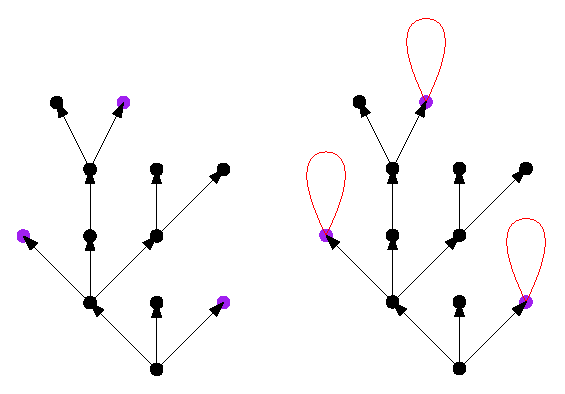
\includegraphics[scale=0.6]{Content/Pictures/black_purple_red_tree.eps}
    \caption{Given a component of $(F^p_n(k),k\geq 1)$ (see left figure), we modify it by sampling independent red Galton-Watson trees with offspring distributed as $Z^+$ and identifying each purple vertex with a root of a red tree. The resulting tree (see right figure) is a Galton-Watson tree, and the resulting forest $(F^{pr}_n(k),k\geq 1)$ is a Galton-Watson forest.}
    \label{fig.blackpurpleredforest}
\end{figure}
The formal procedure is as follows. Suppose we are given $(Y^+(k),S^{+}(k),P_n(k),k\geq 1)$, which encode $(F^p_n(k),k\geq 1)$.
\begin{enumerate}
    \item Let $(Y^{red}(k),k\geq 1)$ be an independent copy of $(Y^+(k),k\geq 1)$. We let $(Y^{red}(k),k\geq 1)$ encode the red pendant subtrees. 
    \item Define $\theta_n(k)=k+\min\{j: Y^{red}(j)=-P_n(k-1)\}-P_n(k-1)$. 
    \item Set $\Lambda_n(k)=\max\{j:\theta_n(j)\leq k\}-P_n(\max\{j:\theta_n(j)\leq k\})$. 
    \item We now define \begin{equation}\label{eq.definitionY^{pr}}(Y^{pr}(k),k\geq 1)=(Y^+(\Lambda_n(k))+Y^{red}(k-\Lambda_n(k)),k\geq 1)\end{equation}
    and we let $(F^{pr}(k),k\geq 1)$ be the Galton-Watson process encoded by $(Y^{pr}(k),k\geq 1)$, in which $P_n(\max\{j:\theta_n(j)\leq k\})$ of the first $k$ vertices are blue, $\Lambda_n(k)$ of the first $k$ vertices are black, and the rest is red. We let $(H^{pr}(k),k\geq 1)$ be the height process corresponding to $(F^{pr}(k),k\geq 1)$.
\end{enumerate}
We claim that the forest consisting of the black and blue vertices in $F^{pr}(\theta_n(k))$ is, by construction, equal to $F^{p}(k)$. Moreover, $(F^{pr}(k),k\geq 1)$ is a Galton-Watson forest. We make the following observations.
\begin{enumerate}
    \item We claim that $$\theta_n(k)=\min\{l: F^p(k)\text{ is a subforest of }F^{pr}(l)\}.$$ Indeed, note that $\min\{j: Y^{red}(j)=-P_n(k-1)\}$ is equal to the number of vertices in the first $P_n(k-1)$ trees in the forest encoded by $Y^{red}$, so $$\min\{j: Y^{red}(j)=-P_n(k-1)\}-P_n(k-1)$$ is equal to the number of red vertices we add to $F^p(k)$. Then, $\theta_n(k)$ is the index in $(F^{pr}(k),k\geq 1)$ of the $k^{th}$ black or purple vertex. 
    \item Note that $\Lambda_n(k)$ is the number of blue vertices amongst the first $k$ vertices. This follows from the fact that $\max\{j:\theta_n(j)\leq k\}$ is the number of blue or purple vertices amongst the first $k$ vertices. 
    \item By the argument above, $(\Lambda_n(k),k\geq 1)$ only takes steps of size $0$ or $1$. Both $(Y^+(k),k\geq 1)$ and $(Y^{red}(k),k\geq 1)$ are random walks with steps distributed as $Z^+-1$, so, by construction, $(Y^{pr}(k),k\geq 1)$ is a random walk with steps distributed as $Z^+-1$, so $(F^{pr}(k),k\geq 1)$ is a Galton-Watson forest with offspring distributed as $Z^+$.
    \item By construction, $(H^{pr}(\theta_n(k)),k\geq 1)$ is the height process corresponding to $(F^p_n(k),k\geq 1)$. Moreover,
   \begin{equation}\label{eq.constructionSp}(S^{+}(k),k\geq 1)=(Y^{pr}(\theta_n(k))-E(\theta_n(k)),k\geq 1),\end{equation}
    where 
    $E(k)$ counts the red children of the $k^{th}$ vertex in $(F^{pr}(k),k\geq 1)$.
\end{enumerate}
Considering the construction above and Corollary \ref{cor.lukasiewiczpathpurplevertices}, in order to prove Proposition \ref{prop.convheightprocesspurple}, it is sufficient to prove the following proposition.
\begin{proposition}\label{prop.heightprocessblackpurplered}
There exists a process $(D_t,t\geq 0)$ such that 
\begin{align*}
    &\left(n^{-1/3}\left[Y^{pr}\left(\theta_n\left(\lfloor n^{2/3}t\rfloor \right)\right)-E\left(\lfloor n^{2/3}t\rfloor \right)\right], n^{-1/3}H^{pr}\left(\theta_n\left(\lfloor n^{2/3}t\rfloor \right)\right),t\geq 0\right)\\
    &\overset{d}{\to}\left(\sigma_+D_t,\frac{2}{\sigma_+}\left(D_t-\inf\left\{D_s,s\leq t\right\}\right),t\geq 0\right)
\end{align*}
in $\D(\R_+,\R)^2$ as $n\to \infty$ and $\left(\frac{2}{\sigma_+}\left(D_t-\inf\left\{D_s,s\leq t\right\}\right),t\geq 0\right)$ is the height process corresponding to $(\sigma_+D_t,t\geq 0)$.
\end{proposition} 
We postpone the proof to Appendix \ref{appendix.heightprocessblackpurplered}. 

\subsection{Applying the measure change to prove Theorem \ref{thm.convoutforest}}\label{subsubsec.convaftermeasurechange}

We will combine the convergence of the measure change under rescaling, which is the content of Lemma \ref{lem:measure-change}, and the convergence of the encoding processes of $(F^p(k),k\geq 1)$, which is the content of Proposition \ref{prop.convheightprocesspurple}, to prove Theorem \ref{thm.convoutforest}.

\begin{proof}[Proof of Theorem \ref{thm.convoutforest}]
Recall that $\hat{P}_n(k)$ denotes the number of purple vertices in $\hat{F}_n(k)$. Set $\hat{I}_n(k)=\min\{\hat{S}^{+}_n(l):l\leq k\}$. Then, as shown in Lemma \ref{lemma.sampleoutforest}, the probability that the $(k+1)^{th}$ vertex in $(\hat{F}_n(k),k\geq 1)$ is purple is given by
$$q_{k+1}:=\frac{\hat{S}^-(k)}{\sum_{i=0}^n D^-_i-k-\hat{I}_n(k)}\one_{\left\{\hat{I}_n(k-1)= \hat{I}_n(k)\right\}}.$$
In order to use the results on $(F^p(k),k\geq 1)$, we would like to replace the term $\sum_{i=0}^n D^-_i$ in the denominator by $\mu n$. Therefore, define a new forest $(\hat{F}'_n(k), k\geq 1)$ in which the probability that the $(k+1)^{th}$ vertex is a purple leaf is
$${q}'_{k+1}:=\frac{\hat{S}^-(k)}{\mu n-k-\hat{I}'_n(k)}\one_{\left\{\hat{I}'_n(k-1)=\hat{I}'_n(k)\right\}},$$
where $\hat{P}'_n(k)$ is the number of purple vertices in $\hat{F}'_n(k)$, and $\hat{I}'_n(k)$ is the number of components in $\hat{F}'_n(k)$. 
We claim that there exists a coupling such that
$$\sum_{i=1}^{\lfloor n^{2/3}T\rfloor }|q_i-q'_i|\overset{p}{\to}0$$
as $n\to \infty$. 
Indeed, by the convergence in Theorem \ref{theorem.convaftermeasurechange}, 
$$\left(n^{-2/3}\sum_{i=1}^{\lfloor n^{2/3}T\rfloor} \hat{D}^n_i\right)_{n>0}$$ is tight. Moreover, with a slight adaptation to the proof of Lemma \ref{lemma.tightnesssurplusedges}, we can show that $\left(n^{-1/3}\hat{P}'_n\left(\lfloor n^{2/3}T\rfloor \right)\right)_{n>0}$ is tight. This, combined with the convergence under rescaling of $(\hat{Y}^+_n(k),k\geq 1)$, implies that also $\left(n^{-1/3}\hat{I}'_n\left(\lfloor n^{2/3}T\rfloor \right)\right)_{n>0}$ is tight.  Since $D^-_1,\dots,D^-_n$ are i.i.d. random variables with mean $\mu$ and finite variance,
$\left(n^{-1/2}\left(\sum_{i=0}^{n-1}D^-_i-\mu n\right)\right)_{n>0}$ is tight. By using the trivial identity $a/b-c/d=(b(a-c)-c(d-b))/bd$, this implies that
$\left(n^{2/3}\max_{k\leq \lfloor n^{2/3}T\rfloor }|q_k-q'_k|\right)_{n>0}$ is tight, which implies that there exists a coupling such that $\left(\max_{k\leq \lfloor n^{2/3}T\rfloor } |\hat{P}_n(k)-\hat{P}'_n(k)|\right)_{n>1}$ and $\left(\max_{k\leq \lfloor n^{2/3}T\rfloor } |\hat{I}_n(k)-\hat{I}'_n(k)|\right)_{n>1}$ are tight, which implies that, again by $a/b-c/d=(b(a-c)-c(d-b))/bd$, 
$\left(n^{5/6}\max_{k\leq \lfloor n^{2/3}T\rfloor }|q_k-q'_k|\right)_{n>0}$ is tight, which implies that 
$$\sum_{i=0}^{\lfloor n^{2/3}T\rfloor }|q_i-q'_i|\overset{p}{\to}0$$
as $n\to \infty$. 
Therefore, under the right coupling, 
$$\P\left(\max_{k\leq \lfloor n^{2/3} T \rfloor}|\hat{P}_n(k)-\hat{P}'(k)|>0\right)\to 0.$$
In other words, we can couple $(\hat{F}_n(k),k\geq 1)$ and $(\hat{F}'_n(k),k\geq 1)$ in such a way that we do not see the difference on the scale that we are interested in. Therefore, we can show convergence under rescaling of the encoding processes of $(\hat{F}'_n(k),k\geq 1)$ instead. To avoid further complicating notation, we will from now on refer to its encoding processes as $$(\hat{S}^{+}_n(k),\hat{H}_n, \hat{S}^-_n(k), \hat{P}_n(k),k\leq \lfloor n^{2/3}T\rfloor).$$ Then, these processes are constructed out of sample paths of $(\hat{Y}^+(k),\hat{Y}^-(k), k\leq \lfloor n^{2/3}T\rfloor )$ and independent randomness in the exact same way as the sample paths of $$({S}_n^{+}(k),{H}_n^+(k),{S}_n^-(k),P_n(k), k \leq \lfloor n^{2/3}T\rfloor )$$ are constructed out of sample paths of $(Y^+(k),Y^-(k), k\leq \lfloor n^{2/3}T\rfloor )$ and independent randomness. 
We will use the following notation:\begin{align*}
    \hat{S}^{+}_{(n)}&:=\left(n^{-1/3}\hat{S}^{+}_n\left(\lfloor n^{2/3} t \right),0\leq t \leq T\right)\\
    \hat{H}_{(n)}&:=\left(n^{-1/3}\hat{H}_n\left(\lfloor n^{2/3} t \right),0\leq t \leq T\right)\\
    \hat{Y}^+_{(n)}&:=\left(n^{-1/3}\hat{Y}^+\left(\lfloor n^{2/3} t \right),0\leq t \leq T\right)\\
     {S}^{+}_{(n)}&:=\left(n^{-1/3}{S}^{+}_n\left(\lfloor n^{2/3} t \right),0\leq t \leq T\right)\\
    {H}^+_{(n)}&:=\left(n^{-1/3}{H}^+_n\left(\lfloor n^{2/3} t \right),0\leq t \leq T\right)\\
    {Y}^+_{(n)}&:=\left(n^{-1/3}{Y}^+\left(\lfloor n^{2/3} t \right),0\leq t \leq T\right).
\end{align*}
Let $f:D([0,T],\R)^3\to \R$ be a bounded, continuous test-function. Then,
\begin{align*}\E\left[f\left(\hat{Y}^+_{(n)}, \hat{S}^+_{(n)},  \hat{H}_{(n)}\right) \right]&= \E\left[ \E\left[\left. f\left(\hat{Y}^+_{(n)},\hat{S}^+_{(n)},  \hat{H}_{(n)}\right)\right|\hat{Y}^+_{(n)}\right]\right]\\&=\E\left[ \Phi(n,\lfloor n^{2/3} T\rfloor)\E\left[\left.f\left(Y^+_{(n)}, S^+_{(n)},  H^+_{(n)}\right)\right| {Y}^+_{(n)}\right]\right]\\&=\E\left[ \Phi(n,\lfloor n^{2/3} T\rfloor)f\left(Y^+_{(n)},S^+_{(n)},  H^+_{(n)}\right)\right],\end{align*}
where we use that $\E\left[\left. f\left(\hat{Y}^+_{(n)},\hat{S}^+_{(n)},  \hat{H}_{(n)}\right)\right|\hat{Y}^+_{(n)}\right]$ is a bounded, adapted function of $\hat{Y}^+_{(n)}$, and that $\Phi(n,\lfloor n^{2/3} t\rfloor)$ is the measure change from ${Y}^+_{(n)}$ to $\hat{Y}^+_{(n)}$. Then, using Lemma \ref{lem:measure-change} and Proposition \ref{prop.convheightprocesspurple}, following the proof of Theorem 4.1 in \cite{conchon--kerjanStableGraphMetric2020} gives us that 
\begin{align*}
    &\E\left[f\left(\hat{Y}^+_{(n)},\hat{S}^+_{(n)},  \hat{H}_{(n)}\right) \right]\\
    &\to \E\left[\Phi(T)f\left(\sigma_+ B_t,\sigma_+ B^+_t,\frac{2}{\sigma_+}R^+_t,0\leq t \leq T\right)\right].
\end{align*}
Since $$(B^+_t,t\geq 0)=\left(B_t-\frac{\nu_-}{2\sigma_+ \mu}t^2,t\geq 0\right),$$
Lemma \ref{lemma.characterizelimitprocess} implies the convergence under rescaling of $(\hat{S}^+_n(k),\hat{H}_n(k),k\geq 0)$. By Proposition \ref{prop.convheightprocesspurple} , $S^{-}_n$ converges in distribution to a deterministic process under scaling, which will not be affected by the measure change. This completes the proof. 
\end{proof}

\subsection{Convergence of the out-forest holds conditionally on the multigraph being simple}
We will now show that the parts of the multigraph we observe up until the timescale in which we are interested are with high probability simple. We will then use an argument by Joseph \cite{josephComponentSizesCritical2014} to show that this implies that Theorem \ref{thm.convoutforest} holds conditional on the resulting multigraph being simple. We let $B_n(k)$ be the number of self-loops and edges created parallel to an existing edge in the same direction as that edge, up until discovery of the $k^{th}$ vertex of $(\hat{F}_n(k),k\geq 1)$. We call these anomalous edges. 
\begin{proposition}\label{prop.anomalousedges}
Suppose $\beta<1$. Then we have
$$\P\left(B_n(\lfloor n^\beta \rfloor)>0\right)\to 0$$
as $n\to \infty$.
\end{proposition}
\begin{remark}
We adapt the proof of Lemma 7.1 of \cite{josephComponentSizesCritical2014} and of Proposition 5.3 of \cite{conchon--kerjanStableGraphMetric2020} to the directed setting. A significant complication is caused by the conditioning on $$\left\{\sum_{i=1}^n D^-_i=\sum_{i=1}^n D^+_i.\right\}.$$ We remark that in both papers, the proof of the aforementioned result is not fully correct, because the authors use a wrong expression for the probability of sampling an anomalous edge. However, the argument below can be adapted to the setting of \cite{josephComponentSizesCritical2014} and \cite{conchon--kerjanStableGraphMetric2020} to yield a correct proof.
\end{remark}
\begin{proof}
Note that we can only show the convergence of the Radon-Nikodym derivative up to time $O(n^{2/3})$, so it is not straightforward to use the measure change to proof results on a time scale $O(n^\beta)$. Therefore, for the proof of this lemma, we will use a different method, that was introduced by Joseph in \cite{josephComponentSizesCritical2014} referred to as \emph{Poissonization}. Let $R_n$ be as before, and conditional on $R_n$, let $D^{0,+}_1,\dots,D^{0,+}_{n-R_n}$ i.i.d.\ random varialbes with the law of $D^+$ conditional on $D^-=0$, and set $S_{n-R_n}=\sum_{i=1}^{n-R_n}$. There is an $L$ such that with high probability, both $R_n$ and $S_{n-R_n}$ are within an interval of width $Ln^{1/2}$ around their mean. We condition on this event. Suppose $R_n=r$ and $S_{n-R_n}=s$, such that the conditioning implies that, in particular, $r=O(n)$. We note that, conditional on $R_n=r$, $(\mathbf{\hat{D}}_{n,1},\dots,\mathbf{\hat{D}}_{r,n})$ (before conditioning on $\sum_{i=1}^nD^-_i=\sum_{i=1}^nD^+_i$) are distributed as the jumps ordered by jump time in a Poisson process $\Pi^0$ with intensity measure $\pi^0$ on $\R_+\times \N^2$ such that $$\pi^0(dt,k_1,k_2)=r\P(D^-=k_1,D^+=k_2|D^->0)k_1\exp(-k_1 t)dt$$
conditional on $\Pi^0(\R,\N,\N)=r$.
The intensity of this process is not constant in $t$, so we perform a time change. Define
$$\cL_{\mathbf{D}}(x,y)=\E\left[\left.\exp(-xD^--yD^+)\right|D^->0 \right],$$
and set 
$$\psi(t)=\left(1-\cL(\cdot,0)\right)^{-1},$$
so that for 
$$\pi_r(dt,k_1,k_2):=\P(D^-=k_1,D^+=k_2)k_1\exp\left(-k_1 \psi(t/r)\right)\psi'(t/r)dt$$
on $(0,r)\times \N^2$, we have that for $t\in (0,r)$, there exists a probability measure $P_t$ on $\N^2$ such that
$$\pi_r(dt,k_1,k_2)=P_t(D^+=k_1,D^+=k_2)dt.$$
This is a trivial adaptation of Lemma 4.1 of \cite{josephComponentSizesCritical2014}. Let ${\Pi}_r$ be a decorated point process with intensity $\pi_r$.  Now, let $\hat{\Pi}_r$ be a random measure, which is a decorated point process with intensity $\pi_r$, conditioned on 
\begin{enumerate}
    \item $N_r:= \hat{\Pi}_r((0,r),\N,\N)=r$, and 
    \item $\Delta_r:=\int_{(0,r)\times \N^2}(k_1-k_2) \hat{\Pi}_r(dt,k_1,k_2)=s$.
\end{enumerate}
Then, the points of $\hat{\Pi}_r$ ordered by time are distributed as $(\mathbf{\hat{D}}_{n,1},\dots,\mathbf{\hat{D}}_{n,r})$ conditional on $\sum_{i=1}^nD^-_i=\sum_{i=1}^nD^+_i$, $R_n=r$ and $S_{n-R_n}=s$. Let $\hat{\pi}^r_t$ be the marginal density of $\hat{\Pi}^r$ at time $t$, so that there is a probability measure $\hat{P}^r_t$ on $\N^2$  and a measure $\lambda^r_t$ on $\R_+$ such that $$\hat{\pi}^r_t(dt,k_1,k_2)=\lambda^r_t(dt)\times \hat{P}^r_t(D^-=k_1, D^+=k_2).$$
Note that due to the conditioning, $\lambda^r_t(dt)$ can be unequal to $dt$. However, we claim that, also after conditioning, with high probability, we will have seen between $n^\beta$ and $3n^\beta$ jumps at time $2n^{\beta}$. Indeed,
\begin{align}\begin{split}\label{eq.numberofjumpsinrandommeasure}\P\left(\left.\Pi_r\left((0,2n^{\beta}),\N,\N\right)\not\in (n^\beta,3n^\beta)\right|\Delta_n=0, N_n=n\right)&\leq \frac{\P\left(\sum_{i=1}^{n^\beta}E_i>2n^{\beta}\text{ or }\sum_{i=1}^{3n^\beta}E_i<2n^{\beta}\right)}{\P(\Delta_r=s, N_r=r)}\\
&=O(n^{1/2}\exp(-n^\beta))\end{split}\end{align}
for $(E_1,E_1,\dots)$ i.i.d. exponential random variables with rate $1$, where the order follows from Cramér's Theorem and the local limit theorem (recall that we conditioned $r$ and $s$ to be at distance $O(n^{1/2})$ from the mean of $R_n$ and $S_{n-R_n}$ respectively). \\
We will use this set-up to show that with high probability, we do not sample anomalous edges in the first $n^\beta$ time steps of the eDFS. We distinguish between the following types of anomalous edges.\\
Self-loops occur when the out-half-edge of a vertex is paired to an in-half-edge of the same vertex.  Let $B^1_n(k)$ be the number of self-loops that are found up to time $k$. For $v$ explored up to time $\lfloor n^\beta\rfloor$, a vertex with in-degree $d^-_v$ and out-degree $d^+_v$, there are $d^-_v d^+_v$ possible combinations of an in-half-edge and an out-half-edge that form a self-loop connected to $v$. Any of these combinations of half-edges is paired with probability bounded above by 
$$\frac{1}{\sum_{i=\lfloor n^\beta \rfloor+1}^n\hat{D}^-_i}.$$
Parallel edges occur when an out-half-edge of a vertex is paired to an in-half-edge of one of its previously explored children. Let $B^2_n(k)$ be the number of parallel edges that are found up to time $k$. For any vertex $v$ with in-degree $d^-_v$, and a parent $p(v)$ with out-degree $d^+_{p(v)}$, there are at most $d^-_v d^+_{p(v)}$ possible combinations of an in-half-edge and an out-half-edge that form a parallel edge from $p(v)$ to $v$. Again, any of these combinations of half-edges is paired with probability bounded above by 
$$\frac{1}{\sum_{i=\lfloor n^\beta \rfloor+1}^n \hat{D}^-_i}.$$
The last type of anomalous edges is a surplus edge with multiplicity greater than 1. Let $B^3_n(k)$ be the number of surplus edges with multiplicity greater than 1 that are found up to time $k$. For a vertex $w$ with out-degree $d^+_w$ and a vertex $v$ with in-degree $d^-_v$, a multiple surplus edge from $w$ to $v$ can only occur if $v$ is discovered before $w$. In that case, there are at most $(d^+_w)^2(d^-_v)^2$ possible pairs of combinations of half-edges, and each of these pairs appears with probability bounded above by
$$\left(\frac{1}{\sum_{i=\lfloor n^\beta \rfloor+1}^n \hat{D}^-_i}\right)^2.$$
Let $p(i)$ denote the index of the parent of the vertex with index $i$. Also, denote $$\cG^n=\sigma\left(\hat{D}^-_1,\hat{D}^+_1,\dots,\hat{D}^-_n,\hat{D}^+_n \right).$$ Then, by a conditional version of Markov's inequality, 

\begin{align*}\P\left(\left.B^1_n(\lfloor n^\beta \rfloor)>0\right| \cG^n \right)&\leq \frac{\sum_{i=1}^{\lfloor n^\beta \rfloor} \hat{D}^-_i\hat{D}^+_i}{\sum_{i=\lfloor n^\beta \rfloor+1}^n \hat{D}^-_i}\wedge 1,\\
\P\left(\left.B^2_n(\lfloor n^\beta \rfloor)>0\right| \cG^n \right)&\leq \frac{\sum_{i=1}^{\lfloor n^\beta \rfloor} \hat{D}^-_i\E\left[\left.\hat{D}^+_{p(i)}\right|\cG^n\right]}{\sum_{i=\lfloor n^\beta \rfloor+1}^n \hat{D}^-_i}\wedge 1,\\
\P\left(\left.B^3_n(\lfloor n^\beta \rfloor)>0\right| \cG^n \right)&\leq \frac{\sum_{i=1}^{\lfloor n^\beta \rfloor}\sum_{j<i} (\hat{D}^+_i)^2 (\hat{D}^-_j)^2 }{\left(\sum_{i=\lfloor n^\beta \rfloor+1}^n \hat{D}^-_i\right)^2 }\wedge 1,\end{align*}
where we note that $p(i)$ is not adapted to $\cG^n$, because ancestral relations in the tree also depend on surplus edges. However, we observe that by the Cauchy-Schwarz inequality,
\begin{align*}\sum_{i=1}^{\lfloor n^\beta \rfloor} \hat{D}^-_i\E\left[\left.\hat{D}^+_{p(i)}\right|\cG^n\right]&\leq \left(\sum_{i=1}^{\lfloor n^\beta \rfloor} (\hat{D}^-_i)^2\right)^{1/2}\left(\sum_{i=1}^{\lfloor n^\beta \rfloor} \E\left[\left.\hat{D}^+_{p(i)}\right|\cG^n\right]^2\right)^{1/2}\\
&\leq\left(\sum_{i=1}^{\lfloor n^\beta \rfloor} (\hat{D}^-_i)^2\right)^{1/2}\left(\sum_{i=1}^{\lfloor n^\beta \rfloor} (\hat{D}^+_i)^3\right)^{1/2}\end{align*}
where the last inequality follows from the conditional Jensen inequality and the fact that a vertex with out-degree $d^+$ that is discovered before time $n^\beta$ is the parent of at most $d^+$ vertices that are discovered before time $n^\beta$.

We will show that \begin{equation}\label{eq.conditionalprobanamolousedges}\P\left(\left.B^1_n(\lfloor n^\beta \rfloor)+B^2_n(\lfloor n^\beta \rfloor)+B^3_n(\lfloor n^\beta \rfloor)>0\right| \cG^n \right)\overset{p}{\to}0\end{equation} as $n\to\infty$. Then, the proposition follows from the bounded convergence theorem. By the observations above, and the fact that $$\sum_{i=\lfloor n^\beta \rfloor+1}^n \hat{D}^-_i=\sum_{i=1}^n D^-_i-\sum_{i=1}^{\lfloor n^\beta \rfloor -1}\hat{D}^-_i,$$ it is sufficient to show that as $n\to \infty$,
\begin{align}
\frac{1}{n}\int_{(0,2n^\beta)\times \N^2}k_1k_2 \hat{\Pi}_r(dt,k_1,k_2)&\overset{p}{\to}0,\label{eq.convergencemomentpointprocess1}\\
\frac{1}{n}\int_{(0,2n^\beta)\times \N^2}k_1 \hat{\Pi}_r(dt,k_1,k_2)&\overset{p}{\to}0,\label{eq.convergencemomentpointprocess2}\\
\frac{1}{n}\int_{(0,2n^\beta)\times \N^2}k_1^2 \hat{\Pi}_r(dt,k_1,k_2)&\overset{p}{\to}0,\label{eq.convergencemomentpointprocess3}\\
\frac{1}{n}\int_{(0,2n^\beta)\times \N^2}k_2^2 \hat{\Pi}_r(dt,k_1,k_2)&\overset{p}{\to}0,\text{ and }\label{eq.convergencemomentpointprocess4}\\
\frac{1}{n}\int_{(0,2n^\beta)\times \N^2}k_2^3 \hat{\Pi}_r(dt,k_1,k_2)&\overset{p}{\to}0.\label{eq.convergencemomentpointprocess5}\end{align}
We will show \ref{eq.convergencemomentpointprocess1}. The proof of the other equations is analogous. \\
We start with the proof of \ref{eq.convergencemomentpointprocess1}. Note that by \eqref{eq.numberofjumpsinrandommeasure}, for $\hat{E}^r_t$ the expectation under $\hat{P}^r_t$, it is sufficient if we show that for some $C$,
\begin{equation}\label{eq.expectationtobound}{\hat{E}}^r_t\left[\hat{D}^-_t\hat{D}^+_t\right]
% :=\frac{\E\left[\int_{\N^2}k_1k_2\hat{\Pi}_n(dt,k_1,k_2)\right]}{\E\left[\int_{\N^2}\hat{\Pi}_n(dt,k_1,k_2)\right]}
<C\end{equation}
for all $n$ and $t<2n^\beta$. We note that
$${\hat{E}}^r_t\left[\hat{D}^-_t\hat{D}^+_t\right]={E}^r_t\left[\hat{D}^-\hat{D}^+| \Delta_r=s, N_r=r\right]={E}^r_t\left[\hat{D}^-\hat{D}^+\frac{\P\left[ \Delta_n=s, N_r=r | \hat{D}^-_t,\hat{D}^+_t\right]}{\P\left[ \Delta_r=s, N_r=r\right]}\right].$$
By the fact that $\Pi_r$ is a decorated point process, we have that for $k_1$, $k_2$ in $\N$, 
$$\P\left[\left. \Delta_r=s, N_r=r \right| \hat{D}^-_t=k_1,\hat{D}^+_t=k_2\right]=\P\left[ \Delta_r=s+k_2-k_1, N_r=r-1 \right],$$
so that, since $N_r\sim \operatorname{Poisson}(r)$, and since on $N_r=r-1$ (resp. $N_r=r$),  $\Delta_r-s$ is the sum of $r-1$ (resp. $r$) i.i.d. random variables with finite variance and mean at most $O(r^{-1/2})$, we observe that 
\begin{align*}
    \P\left[ \Delta_r=s, N_r=r | \hat{D}^-_t=k_1,\hat{D}^+_t=k_2\right]&=\omega(r^{-1/2})\text{, and}\\
    \P\left[ \Delta_r=s, N_r=r \right]&=O(r^{-1/2})
\end{align*} for any $k_1$, $k_2$. Therefore, there exists a $C'$ such that
$$\frac{\P\left[ \Delta_r=s, N_r=r | \hat{D}^-_t=k_1,\hat{D}^+_t=k_2\right]}{\P\left[ \Delta_r=s, N_r=r\right]}<C'$$
for all $k_1$, $k_2$, $t$ and $n$. If we show that for some $C''$ $${E}^r_t\left[\hat{D}^-\hat{D}^+\right]<C''$$ for all $r$ in the interval that we consider and all $t<2n^\beta$,  \eqref{eq.expectationtobound} follows. We note that by definition of $\pi_r(dt,k_1,k_1)$, 
$${E}^r_t\left[\hat{D}^-\hat{D}^+\right]=\frac{\frac{d^3}{dx^2 dy}\cL_{\mathbf{D}}(x,y)|_{(\psi(t/r),0)}}{\frac{d}{dx}\cL_{\mathbf{D}}(x,y)|_{(\psi(t/r),0)}}.$$
Careful analysis of $\cL_{\mathbf{D}}(x,y)$ and $\psi(s)$ implies that this quantity is bounded uniformly for all $r$ in the interval that we consider and all $t\in(0,2n^\beta)$. We refer the reader to the proof of Lemma A.1 in \cite{josephComponentSizesCritical2014} for the details of a similar argument in the undirected setting. Then, \eqref{eq.expectationtobound} follows. \\
By applying the same techniques, \eqref{eq.convergencemomentpointprocess2}, \eqref{eq.convergencemomentpointprocess3}, \eqref{eq.convergencemomentpointprocess4} and  \eqref{eq.convergencemomentpointprocess5} follow as well, which proves the statement.

% Note that we can only show the convergence of the Radon-Nikodym derivative up to time $O(n^{2/3})$, so it is not straightforward to use the measure change to proof results on a time scale $O(n^\beta)$. Therefore, for the proof of this lemma, we will use a different method, that was introduced by Joseph in \cite{josephComponentSizesCritical2014} referred to as \emph{Poissonization}. We note that $(\mathbf{\hat{D}}_{n,1},\dots,\mathbf{\hat{D}}_{n,n})$ (before conditioning on $\sum_{i=1}^nD^-_i=\sum_{i=1}^nD^+_i$) are distributed as the jumps ordered by jump time in a Poisson process $\Pi^0$ with intensity measure $\pi^0$ on $\R_+\times \N^2$ such that $$\pi^0(dt,k_1,k_2)=n\P(D^-=k_1,D^+=k_2)k_1\exp(-k_1 t)dt$$
% conditionally on $\Pi^0(\R,\N,\N)=n$.
% The intensity of this process is not constant in $t$, so we perform a time change. Define
% $$\cL_{\mathbf{D}}(x,y)=\E\left[\exp(-xD^--yD^+)\right],$$
% and set 
% $$\psi(t)=\left(1-\cL(\cdot,0)\right)^{-1},$$
% so that for 
% $$\pi_n(dt,k_1,k_2):=\P(D^-=k_1,D^+=k_2)k_1\exp\left(-k_1 \psi(t/n)\right)\psi'(t/n)dt$$
% on $(0,n)\times \N^2$, we have that for $t\in (0,n)$, there exists a probability measure $P_t$ on $\N^2$ such that
% $$\pi_n(dt,k_1,k_2)=P_t(D^+=k_1,D^+=k_2)dt.$$
% This is a trivial adaptation of Lemma 4.1 of \cite{josephComponentSizesCritical2014}. Let ${\Pi}_n$ be a decorated point process with intensity $\pi_n$. Now, let $\hat{\Pi}_n$ be a random measure, which is a decorated point process with intensity $\pi_n$, conditionally on 
% \begin{enumerate}
%     \item $N_n:=\hat{\Pi}_n((0,n),\N,\N)=n$, and 
%     \item $\Delta_n:=\int_{(0,n)\times \N^2}(k_1-k_2)\hat{\Pi}_n(dt,k_1,k_2)=0$.
% \end{enumerate}
% Then, the points of $\hat{\Pi}_n$ ordered by time are distributed as $(\mathbf{\hat{D}}_{n,1},\dots,\mathbf{\hat{D}}_{n,n})$ conditionally on $\sum_{i=1}^nD^-_i=\sum_{i=1}^nD^+_i$. Let $\hat{\pi}^n_t$ be the marginal density of $\hat{\Pi}^n$ at time $t$, so that there is a probability measure $\hat{P}^n_t$ on $\N^2$  and a measure $\lambda^n_t$ on $\R_+$ such that $$\hat{\pi}^n_t(dt,k_1,k_2)=\lambda^n_t(dt)\times \hat{P}^n_t(D^-=k_1, D^+=k^2).$$
% Note that due to the conditioning, $\lambda^n_t(dt)$ can be unequal to $dt$. However, we claim that, also after conditioning, with high probability, we will have seen between $n^\beta$ and $3n^\beta$ jumps at time $2n^{\beta}$. Indeed,
% \begin{align}\begin{split}\label{eq.numberofjumpsinrandommeasure}\P\left(\left.\Pi_n\left((0,2n^{\beta}),\N,\N\right)\not\in (n^\beta,3n^\beta)\right|\Delta_n=0, N_n=n\right)&\leq \frac{\P\left(\sum_{i=1}^{n^\beta}E_i>2n^{\beta}\text{ or }\sum_{i=1}^{3n^\beta}E_i<2n^{\beta}\right)}{\P(\Delta_n=0, N_n=n)}\\
% &=O(n^{1/2}\exp(-n))\end{split}\end{align}
% for $(E_1,E_1,\dots)$ i.i.d. exponential random variables with rate $1$, where the order follows from Cramér's Theorem and the local limit theorem. \\
% We will use this set-up to show that with high probability, we do not sample anomalous edges in the first $n^\beta$ time steps of the eDFS. We distinguish between the following types of anomalous edges.\\
% Self-loops occur when the out-half-edge of a vertex is paired to an in-half-edge of the same vertex.  Let $B^1_n(k)$ be the number of self-loops that are found up to time $k$. For $v$ explored up to time $\lfloor n^\beta\rfloor$, a vertex with in-degree $d^-_v$ and out-degree $d^+_v$, there are $d^-_v d^+_v$ possible combinations of an in-half-edge and an out-half-edge that form a self-loop connected to $v$. Any of these combinations of half-edges is paired with probability bounded above by 
% $$\frac{1}{\sum_{i=\lfloor n^\beta \rfloor+1}^n\hat{D}^-_i}.$$
% Parallel edges occur when an out-half-edge of a vertex is paired to an in-half-edge of one of its previously explored children. Let $B^2_n(k)$ be the number of parallel edges that are found up to time $k$. For any vertex $v$ with in-degree $d^-_v$, and a parent $p(v)$ with out-degree $d^+_{p(v)}$, there are at most $d^-_v d^+_{p(v)}$ possible combinations of an in-half-edge and an out-half-edge that form a parallel edge from $p(v)$ to $v$. Again, any of these combinations of half-edges is paired with probability bounded above by 
% $$\frac{1}{\sum_{i=\lfloor n^\beta \rfloor+1}^n \hat{D}^-_i}.$$
% The last type of anomalous edges is a surplus edge with multiplicity greater than 1. Let $B^3_n(k)$ be the number of surplus edges with multiplicity greater than 1 that are found up to time $k$. For a vertex $w$ with out-degree $d^+_w$ and a vertex $v$ with in-degree $d^-_v$, a multiple surplus edge from $w$ to $v$ can only occur if $v$ is discovered before $w$. In that case, there are at most $(d^+_w)^2(d^-_v)^2$ possible pairs of combinations of half-edges, and each of these pairs appears with probability bounded above by
% $$\left(\frac{1}{\sum_{i=\lfloor n^\beta \rfloor+1}^n \hat{D}^-_i}\right)^2.$$
% Let $p(i)$ denote the index of the parent of the vertex with index $i$. Also, denote $$\cG^n=\sigma\left(\hat{D}^-_1,\hat{D}^+_1,\dots,\hat{D}^-_n,\hat{D}^+_n \right).$$ Then, by a conditional version of Markov's inequality, 

% \begin{align*}\P\left(\left.B^1_n(\lfloor n^\beta \rfloor)>0\right| \cG^n \right)&\leq \frac{\sum_{i=1}^{\lfloor n^\beta \rfloor} \hat{D}^-_i\hat{D}^+_i}{\sum_{i=\lfloor n^\beta \rfloor+1}^n \hat{D}^-_i}\wedge 1,\\
% \P\left(\left.B^2_n(\lfloor n^\beta \rfloor)>0\right| \cG^n \right)&\leq \frac{\sum_{i=1}^{\lfloor n^\beta \rfloor} \hat{D}^-_i\E\left[\left.\hat{D}^+_{p(i)}\right|\cG^n\right]}{\sum_{i=\lfloor n^\beta \rfloor+1}^n \hat{D}^-_i}\wedge 1,\\
% \P\left(\left.B^3_n(\lfloor n^\beta \rfloor)>0\right| \cG^n \right)&\leq \frac{\sum_{i=1}^{\lfloor n^\beta \rfloor}\sum_{j<i} (\hat{D}^+_i)^2 (\hat{D}^-_j)^2 }{\left(\sum_{i=\lfloor n^\beta \rfloor+1}^n \hat{D}^-_i\right)^2 }\wedge 1,\end{align*}
% where we note that $p(i)$ is not adapted to $\cG^n$, because ancestral relations in the tree also depend on surplus edges. However, we observe that by the Cauchy-Schwarz inequality,
% \begin{align*}\sum_{i=1}^{\lfloor n^\beta \rfloor} \hat{D}^-_i\E\left[\left.\hat{D}^+_{p(i)}\right|\cG^n\right]&\leq \left(\sum_{i=1}^{\lfloor n^\beta \rfloor} (\hat{D}^-_i)^2\right)^{1/2}\left(\sum_{i=1}^{\lfloor n^\beta \rfloor} \E\left[\left.\hat{D}^+_{p(i)}\right|\cG^n\right]^2\right)^{1/2}\\
% &\leq\left(\sum_{i=1}^{\lfloor n^\beta \rfloor} (\hat{D}^-_i)^2\right)^{1/2}\left(\sum_{i=1}^{\lfloor n^\beta \rfloor} (\hat{D}^+_i)^3\right)^{1/2}\end{align*}
% where the last inequality follows from the conditional Jensen inequality and the fact that a vertex with out-degree $d^+$ that is discovered before time $n^\beta$ is the parent of at most $d^+$ vertices that are discovered before time $n^\beta$.

% We will show that \begin{equation}\label{eq.conditionalprobanamolousedges}\P\left(\left.B^1_n(\lfloor n^\beta \rfloor)+B^2_n(\lfloor n^\beta \rfloor)+B^3_n(\lfloor n^\beta \rfloor)>0\right| \cG^n \right)\overset{p}{\to}0\end{equation} as $n\to\infty$. Then, the proposition follows from the bounded convergence theorem. By the observations above, and the fact that $$\sum_{i=\lfloor n^\beta \rfloor+1}^n \hat{D}^-_i=\sum_{i=1}^n D^-_i-\sum_{i=1}^{\lfloor n^\beta \rfloor -1}\hat{D}^-_i,$$ it is sufficient to show that as $n\to \infty$,
% \begin{align}
% \frac{1}{n}\int_{(0,2n^\beta)\times \N^2}k_1k_2\hat{\Pi}_n(dt,k_1,k_2)&\overset{p}{\to}0,\label{eq.convergencemomentpointprocess1}\\
% \frac{1}{n}\int_{(0,2n^\beta)\times \N^2}k_1\hat{\Pi}_n(dt,k_1,k_2)&\overset{p}{\to}0,\label{eq.convergencemomentpointprocess2}\\
% \frac{1}{n}\int_{(0,2n^\beta)\times \N^2}k_1^2\hat{\Pi}_n(dt,k_1,k_2)&\overset{p}{\to}0,\label{eq.convergencemomentpointprocess3}\\
% \frac{1}{n}\int_{(0,2n^\beta)\times \N^2}k_2^2\hat{\Pi}_n(dt,k_1,k_2)&\overset{p}{\to}0,\text{ and }\label{eq.convergencemomentpointprocess4}\\
% \frac{1}{n}\int_{(0,2n^\beta)\times \N^2}k_2^3\hat{\Pi}_n(dt,k_1,k_2)&\overset{p}{\to}0.\label{eq.convergencemomentpointprocess5}\end{align}
% We will show \ref{eq.convergencemomentpointprocess1}. The proof of the other equations is analogous. \\
% We start with the proof of \ref{eq.convergencemomentpointprocess1}. Note that by \eqref{eq.numberofjumpsinrandommeasure}, for $\hat{E}^n_t$ the expectation under $\hat{P}^n_t$, it is sufficient if we show that for some $C$,
% \begin{equation}\label{eq.expectationtobound}{\hat{E}}^n_t\left[\hat{D}^-_t\hat{D}^+_t\right]
% % :=\frac{\E\left[\int_{\N^2}k_1k_2\hat{\Pi}_n(dt,k_1,k_2)\right]}{\E\left[\int_{\N^2}\hat{\Pi}_n(dt,k_1,k_2)\right]}
% <C\end{equation}
% for all $n$ and $t<2n^\beta$. We note that
% $${\hat{E}}^n_t\left[\hat{D}^-_t\hat{D}^+_t\right]={E}^n_t\left[\hat{D}^-\hat{D}^+| \Delta_n=0, N_n=n\right]={E}^n_t\left[\hat{D}^-\hat{D}^+\frac{\P\left[ \Delta_n=0, N_n=n | \hat{D}^-_t,\hat{D}^+_t\right]}{\P\left[ \Delta_n=0, N_n=n\right]}\right].$$
% By the fact that $\Pi_n$ is a decorated point process, we have that for $k_1$, $k_2$ in $\N$, 
% $$\P\left[\left. \Delta_n=0, N_n=n \right| \hat{D}^-_t=k_1,\hat{D}^+_t=k_2\right]=\P\left[ \Delta_n=k_2-k_1, N_n=n-1 \right],$$
% so that, since $N_n\sim \operatorname{Poisson}(n)$, and since on $N_n=n-1$ (resp. $N_n=n$),  $\Delta_n$ is the sum of $n-1$ (resp. $n$) i.i.d. mean $0$ random variables with finite variance, there exists a $C'$ such that
% $$\frac{\P\left[ \Delta_n=0, N_n=n | \hat{D}^-_t=k_1,\hat{D}^+_t=k_2\right]}{\P\left[ \Delta_n=0, N_n=n\right]}<C'$$
% for all $k_1$, $k_2$, $t$ and $n$. Therefore, if we show that for some $C''$ $${E}^n_t\left[\hat{D}^-\hat{D}^+\right]<C''$$ for all $n$ and $t<2n^\beta$,  \eqref{eq.expectationtobound} follows. We note that by definition of $\pi_n(dt,k_1,k_1)$, 
% $${E}^n_t\left[\hat{D}^-\hat{D}^+\right]=\frac{\frac{d^3}{dx^2 dy}\cL_{\mathbf{D}}(x,y)|_{(\psi(t/n),0)}}{\frac{d}{dx}\cL_{\mathbf{D}}(x,y)|_{(\psi(t/n),0)}}.$$
% By definition of $\cL_{\mathbf{D}}(x,y)$ and $\psi(s)$, we find that 
% \begin{align*}\frac{d^3}{dx^2 dy}\cL_{\mathbf{D}}(x,y)_{(s,0)}&=-\E[(D^-)^2D^+]+o(1),\\
% \frac{d}{dx}\cL_{\mathbf{D}}(x,y)_{(s,0)}&=-\E[D^-]+o(1)\text{, and}\\
% \psi(s)&=\frac{s}{\mu}+o(s)\end{align*}
% as $s\to 0$. We refer the reader to the proof of Lemma A.1 in \cite{josephComponentSizesCritical2014} for the details of a similar argument in the undirected setting. This implies that 
% $${E}^n_t\left[\hat{D}^-\hat{D}^+\right]=\frac{\E[(D^-)^2D^+]}{\E[D^-]}+o(1)$$
% uniformly in all $t\leq 2n^\beta$, and \eqref{eq.expectationtobound} follows. \\
% By applying the same techniques, \eqref{eq.convergencemomentpointprocess2}, \eqref{eq.convergencemomentpointprocess3}, \eqref{eq.convergencemomentpointprocess4} and  \eqref{eq.convergencemomentpointprocess5} follow as well, which proves the statement.


\end{proof}
\begin{corollary}
 Theorem \ref{thm.convoutforest} holds conditionally on the resulting multigraph being simple. 
\end{corollary}
\begin{proof}
Let $\rho(n)=\inf\{k\geq 1:B_n(k)>0\}$, and note that the event that the multigraph formed by the configuration model on $n$ vertices is simple is equal to $\{\rho(n)=\infty\}$. Proposition \ref{prop.anomalousedges} shows that we do not observe any anomalous edges far beyond the timescale in which we explore the largest components of the out-forest. This allows us to conclude that all of the results we prove using the exploration up to time $O(n^{2/3})$ are also true conditioned on $\{\rho(n)=\infty\}$. This follows from the proof of Theorem 3.2 in \cite{josephComponentSizesCritical2014}.
\end{proof}
All results that follow are obtained by studying the exploration up to time $O(n^{2/3})$, so will also be true conditional on the resulting directed multigraph being simple.


\input{Content/Sections/Convergence of SSC}
\section*{Acknowledgements}
The authors would like to thank Christina Goldschmidt and Robin Stephenson for many fruitful discussions, and for kindly allowing us to use some of their figures, and Igor Kortchemski for his advice on local limit theorems. Finally, the authors would like to thank an anonymous referee for very thorough reading of the paper and for many useful comments.

\section*{Declarations}

\begin{itemize}
    \item The first author, Serte Donderwinkel, has been supported by a Clarendon Scholarship from the Clarendon Fund.
    \item The second author, Zheneng Xie, has been supported by the EPSRC Centre for Doctoral Training in Mathematics of Random Systems: Analysis, Modelling and Simulation (EP/S023925/1).
    \item  Data sharing not applicable to this article as no datasets were generated or analysed during the current study.
\end{itemize}


\appendix
\input{Content/Sections/Appendix convergence height process}
\section{Multivariate triangular local limit theorem}
\label{chap:llt}

For an i.i.d.\ sequence $\vX_1, \ldots, \vX_n$ of random variables, central limit theorems address probabilities of the form
\begin{equation*}
    \P\Big( n^{-\alpha} \textstyle \sum_{i=1}^n (\vX_i - \E[\vX]) \in A \Big).
\end{equation*}
where the $\alpha > 0$ is chosen such that the above probabilities converge to a sensible limit and $A$ is some Borel subset. More abstractly, the $\alpha$ is chosen so that $n^{-\alpha} \sum_{i=1} (\vX_i - \E[\vX])$ converges to a stable law. On the other hand local limit theorems address probabilities of the form
\begin{equation*}
    \P\Big( \textstyle \sum_{i=1}^n (\vX_i - \E[\vX]) \in A \Big).
\end{equation*}
without the $n^{-\alpha}$ scaling. Such probabilities are going to decay to 0, but we can still make statements quantifying how they decay to 0, utilizing the density of the limiting stable distribution for the central limit theorem. Local limit theorems are what we are going to need to know the asymptotic behaviour of
\begin{equation*}
    \P(\Delta_n = 0) = \P\Big(\textstyle\sum_{i=1}^n (D_i^- - D_i^+) = 0\Big).
\end{equation*}
In fact to prove \cref{lem:measure-change} we will need to introduce a sequence of exponentially tilted measures $\P_n$ and thus require a local limit theorem for i.i.d.\ triangular arrays. We will also need to simultaneously control the behaviour of a separate sum and thus we need a bivariate local limit theorem.

Historically, \citet{gnedenkoLocalLimitTheorem1948} covers the stable case in one dimension. For multidimensional random variables, \citet{rvavceva1962domains} covers the lattice case and \citet{stoneLocalLimitTheorem1965} covers the non-lattice case. \citet{doneyBivariateLocalLimit1991} proves a local limit theorem for the bivariate case which allows each component to use a different scaling. A local limit theorem specifically for integer valued random vectors is covered by \citet{gamkrelidzeLocalLimitTheorem2015}.

\citet{jainLowerTailProbability1987} prove a triangular local limit theorem for one dimensional random variables converging to a stable limit. In the one-dimensional case where the random variables possess densities, \citet{korchinskyLocalLimitTheorem2007} address more general non i.i.d.\ triangular arrays where the distribution can vary across rows.

For such more general i.i.d.\ triangular arrays, \citet{chagantyMultidimensionalLargeDeviation1986} prove a local limit theorem in the multivariate case under the assumption that the moment generating functions of the sums are holomorphic. This builds upon work done by \citet{richterLocalLimitTheorems1957,richterMultiDimensionalLocalLimit1958} for the non-triangular case.

Unfortunately the assumptions required to apply the results in the literature are too restrictive for use in our case. In particular we don't assume that our random variables have finite fourth moments, and therefore a Cramér type assumption is too restrictive. Instead it will turn out that the common distribution for each row of our i.i.d.\ triangular array will be converging to the non-tilted case. We will utilize this, along with a uniform integrability type criterion, to prove a general multivariate local limit theorem for lattice valued random variables.

\subsection{Lattices}

\begin{figure}[htbp]
    \centering
    \includegraphics[width=\textwidth]{Content/Pictures/lattice.eps}
    \caption{A lattice with three possible choices of fundamental region shaded}
    \label{fig:lattice}
\end{figure}

Before we state the theorem, we introduce some definitions and theory about lattices. This section will borrow heavily from the textbook by \citet{schrijverTheoryLinearInteger1998}. Suppose we are working in the space $\R^d$. Then a set $\lattice$ is a \emph{lattice} if there exists a basis $\{\va_1, \ldots, \va_d\}$ of $\R^d$ such that
\begin{equation*}
    \lattice = \left\{ \sum_{i=1}^d n_i \va_i : (n_1, \ldots, n_d) \in \Z^d \right\}.
\end{equation*}
The basis can be summarised by the $n \times n$ matrix $A$ with columns $\va_1, \ldots, \va_d$, meaning $A_{ij} = a_i^{(j)}$. Then $\{\va_1, \ldots, \va_d\}$ is a basis of $\R^d$ if and only if $A$ is invertible. 

The vectors $\va_1, \ldots, \va_d$ define a $d$-dimensional parallelepiped
\begin{equation*}
    \Bigg\{\sum_{i=1}^d \lambda_i \va_i : (\lambda_1, \ldots, \lambda_d) \in [0, 1]^d \Bigg\}
\end{equation*}
which is sometimes called the \emph{fundamental region} of the lattice. The choice of basis generating a lattice $\lattice$ is not unique. This can be seen in \cref{fig:lattice} where three different choices of the fundamental region are drawn. It turns out two matrices correspond to the same lattice if and only if they are obtainable from each other through multiplication by a unimodular matrix. A square matrix $U$ is \emph{unimodular} if it has integer entries and has determinant $\pm 1$. \cite[Theorem 4.3]{schrijverTheoryLinearInteger1998} shows that the inverse of a unimodular matrix will also be unimodular, and in particular also has integer entries. The following is then a rephrasing of \cite[Corollary 4.3a]{schrijverTheoryLinearInteger1998}:
\begin{lemma}
    Let $A$ and $B$ be invertible matrices. Then the columns of $A$ and the columns of $B$ generate the same lattice if and only if there exists a unimodular matrix $U$ such that $A = UB$.
\end{lemma}
Suppose a lattice $\lattice$ is generated by the columns of $A$. Define
\begin{equation*}
    \det(\lattice) = \abs{\det(A)}.
\end{equation*}
Then the preceding lemma shows this is well defined even though the choice of $A$ is not unique. The quantity $\det(\lattice)$ is the volume of any choice of the fundamental region.

A canonical choice of matrix generating a lattice is obtainable when the points of the lattice are rational. An invertible matrix $B$ is in \emph{Hermite normal form} if it is lower triangular with non-negative entries. Then the following is a rephrasing of \cite[Corollary 4.3b]{schrijverTheoryLinearInteger1998}:
\begin{lemma}
    Let $A$ be an invertible matrix with rational entries. Then there exists a unique unimodular matrix $U$ such that $UA$ is in Hermite normal form.
\end{lemma}
This gives us the following corollary:
\begin{lemma}
    \label{lem:zd-triangular}
    Suppose $\lattice \subset \Z^d$ is a lattice. Then there exists a lower triangular matrix
    \begin{equation*}
        A = \begin{pmatrix}
            p_1 & & & 0 \\
            p_{2,1} & \ddots & & \\
            \vdots & \ddots & \ddots & \\
            p_{d,1} & \cdots & p_{d, d-1} & p_d
        \end{pmatrix}
    \end{equation*}
    with non-negative integer entries such that $\lattice$ is generated by the columns of $A$.
\end{lemma}

We say a $\R^d$-valued random variable $\vX$ is \emph{non-degenerate} if $\vX$ is not supported in a $(d-1)$-dimensional affine subspace of $\R^d$. Further $\vX$ is \emph{lattice valued} if there a translation of a lattice containing the support of $\vX$.

If $\vX$ is non-degenerate and lattice valued, we wish to define the smallest lattice on which $\vX$ lives. Let $\cS$ be the support of $\vX$ and fix an arbitrary $\vc \in \cS$. Then the \emph{main lattice} of $\vX$ is the smallest lattice containing $\cS - \vc$. Since $X$ is non-degenerate, such a lattice is unique and given by 
\begin{equation*}
    \lattice = \Bigg\{
        \sum_{i=1}^m k_i (\vx_i - \vc) :
        \text{$m \geq 1$ and $k_i \in \Z, \vx_i \in \cS$ for all $i = 1, \ldots, m$}
    \Bigg\}.
\end{equation*}
The strong aperiodicity condition we imposed on $D^- - D^+$ in \cref{chap:directed-configuration-model} can then be stated as saying $D^- - D^+$ has main lattice $\Z$.

The main lattice of $\vX$ is related to the periodicity of its characteristic function. The following lemma is an adaptation of \cite[P.67, T1]{spitzerPrinciplesRandomWalk1964}.
\begin{lemma}
    \label{lem:cf-periodicity}
    Suppose the main lattice of $\vX$ is $\Z^d$ and let $\phi$ be the characteristic function of $\vX$, such that $\phi(\vu) = e^{i \vu \cdot \vX}$. Then $\abs{\phi(\vu)} = 1$ if and only if every coordinate of $\vu$ is a multiple of $2 \pi$.
\end{lemma}
\begin{proof}
    If every coordinate of $\vu$ is a multiple of $2\pi$ then $\vu \cdot \vX$ has support in $t + 2 \pi \Z$ for some $t \in \R$. Therefore $e^{i\vu \cdot \vX}$ is constant and therefore $\abs{\phi(\vu)} = 1$.
    
    For the converse, by Jensen's inequality
    \begin{equation*}
        \abs{\E[e^{i \vu \cdot \vX}]} \leq \E[\abs{e^{i\vu \cdot \vX}}] = 1.
    \end{equation*}
    More importantly to achieve equality, it must be the case that $e^{i \vu \cdot \vX}$ is almost surely constant. Therefore there exists $t \in \R$ such that
    \begin{equation*}
        \vu \cdot \vx \in t + 2 \pi \Z
    \end{equation*}
    for all $\vx \in \cS$. Then fixing an arbitrary $\vc \in \cS$,
    \begin{equation*}
        \vu \cdot (\vx - \vc) \in 2 \pi \Z
    \end{equation*}
    for all $\vx \in \cS$. Since the fundamental lattice of $\vX$ is $\Z^d$, there exists $\vx_1, \ldots, \vx_m \in \cS$ and $k_1, \ldots, k_m \in \Z$ such that
    \begin{equation*}
        \sum_{i=1}^m k_i (\vx_i - \vc) = (1, 0, \ldots, 0).
    \end{equation*}
    Therefore
    \begin{equation*}
        u^{(1)} = \sum_{i=1}^m k_i \vu \cdot (\vx_i - \vc) \in 2 \pi \Z.
    \end{equation*}
    Repeating this argument for the other coordinates of $\vu$ shows all coordinates of $\vu$ are multiples of $2 \pi$.
\end{proof}


\subsection{Triangular local limit theorem}

Throughout this chapter $\norm{\vu}$, for $\vu \in \R^d$, will denote the Euclidean norm
\begin{equation*}
    \norm{\vu} = \Big( \textstyle \sum_{i=1}^d \big\{ u^{(i)} \big\}^2 \Big)^{1/2}.
\end{equation*}

\begin{theorem}
    \label{thm:multi-triangular-llt}
    For each $n \geq 1$ let $\vX_n$ be an $\R^d$ valued random variable and
    \begin{equation*}
        \vX_{n, 1}, \vX_{n, 2}, \ldots, \vX_{n, n}  
    \end{equation*}
    be i.i.d.\ copies of $\vX_n$. Assume that the following holds:
    \begin{enumerate}
        \item There exists a non-degenerate $\R^d$-valued random variable $\vX$ such that
            \begin{equation*}
                \vX_n \todist \vX \quad \text{as $n \to \infty$.}
            \end{equation*} 
        \item For all $n$, $\vX_n$ and $\vX$ have a common main lattice $\lattice$.
        \item $(\norm{\vX_n}^2)_{n \geq 1}$ is a uniformly integrable sequence of random variables. Explicitly
            \begin{equation}
                \label{eq:ui-condition}
                \lim_{L \to \infty} \sup_n \E\left[
                    \norm{\vX_n}^2
                    \one \left\{ \norm{\vX_n}^2 > L \right\}
                \right] = 0.
            \end{equation}
    \end{enumerate}
    Then $\vX$ has finite second moment. Also if $\vc_n$ is defined such that $\vc_n + \lattice$ contains the support of $\sum_{i=1}^n \vX_{n, i}$ then uniformly for $\vy \in \vc_n + \lattice$
    \begin{equation*}
        \P\Big(
            \textstyle \sum_{i=1}^n \vX_{n, i} = \vy
        \Big)
        = n^{-d/2} \det(\lattice) f\left( \vx_n \right) + \littleo \left( n^{-d/2} \right)
        \quad \text{where} \quad
        \vx_n = \frac{\vy - n \E[\vX_n]}{\sqrt{n}}
    \end{equation*}
    and $f$ is the density of a $N(0, \cov(\vX))$ distribution. This means that
    \begin{equation*}
        \lim_{n \to \infty} \sup_{\vy \in \vc_n + \lattice} \abs*{
            n^{d/2} \P\Big( \textstyle \sum_{i=1}^n \vX_{n, i} = \vy \Big)
            - \det(\lattice) f(\vx_n)
        } = 0.
    \end{equation*}
\end{theorem}

We now make a few remarks. Firstly $\cov(\vX)$ is non-degenerate, meaning it is invertible, since we assume that $\vX$ is non-degenerate. In particular this ensures $N(0, \cov(\vX))$ has a density $f$, explicitly given by
\begin{equation*}
    f(\vx) = \frac{1}{\sqrt{(2 \pi)^d \det(\cov(\vX))}}
    \exp \Bigg(
        -\frac{1}{2} \vx \cdot \cov(\vX)^{-1} \vx
        \Bigg).
\end{equation*}

Secondly, since the $\vX_1, \vX_2, \ldots$ do not necessarily live in the same probability space we should not technically refer to the sequence $(\norm{\vX}_n^2)_{n \geq 1}$ as uniformly integrable. However the condition in \cref{eq:ui-condition} is still well defined.

Finally, while the local limit theorem holds for all $\vy$ on the appropriate lattice, the error term will dominate if $\vy$ deviates too far from the mean of $\sum_{i=1}^n \vX_i$. Specifically consider a sequence $\vy_n$ such that
\begin{equation*}
    \norm{\vy_n - n \E[\vX_n]} = \omega(\sqrt{n}).
\end{equation*}
Let $\maxeval$ be the maximum eigenvalue of $\cov(\vX)$. Then
\begin{equation*}
    \bigg( \frac{\vy_n - n \E[\vX_n]}{\sqrt{n}} \bigg)
    \cdot \cov(\vX)^{-1} 
    \bigg( \frac{\vy_n - n \E[\vX_n]}{\sqrt{n}} \bigg)
    \geq \frac{1}{\maxeval} \frac{\norm{\vy_n - n\E[\vX_n]}^2}{n} \to \infty
\end{equation*}
as $n \to \infty$. Thus the local limit theorem only tells us that 
\begin{equation*}
    \P\Big( \textstyle \sum_{i=1}^n \vX_i = \vy_n \Big) = \littleo\Big( n^{-d/2} \Big)
\end{equation*}
meaning we lose the precise characterisation of the leading order term in how this probability decays.

Before we prove our main theorem, we first prove a series of lemmas. Firstly we show the condition in \cref{eq:ui-condition} still holds when we centre the random variables.
\begin{lemma}
    \label{lem:ui-mean-center}
    Suppose we are in the setting of \cref{thm:multi-triangular-llt}. Define $\hat{\vX}_n = \vX_n - \E[\vX_n]$. Then
    \begin{equation*}
        \lim_{L \to \infty} \sup_n \E \left[
            \norm{\hat{\vX}_n}^2
            \one \left\{ \norm{\hat{\vX}_n}^2 > L \right\}
        \right] = 0.
    \end{equation*}
\end{lemma}
\begin{proof}
    The condition in \cref{eq:ui-condition} shows that $M = \sup_n \E[\norm{X_n}^2] < \infty$. By Jensen's inequality, $\sup_n \norm{\E[\vX_n]}^2 \leq M$. Then
    \begin{align*}
        \norm{\hat{\vX}_n}^2 = \norm{\vX_n - \E[\vX_n]}^2
        &\leq 2 \norm{\vX_n}^2 + 2 \norm{\E[\vX_n]}^2 \\
        &\leq 2 \norm{\vX_n}^2 + 2M. \\
    \end{align*}
    Therefore
    \begin{align*}
        \sup_n \E \left[
            \norm{\hat{\vX}_n}^2
            \one \left\{ \norm{\hat{\vX}_n}^2 > L \right\}
        \right]
        &\leq 2 \sup_n \E\Big[\norm{\vX_n}^2 \one \left\{ \norm{\vX_n}^2 \geq \tfrac{1}{2} L - M\right\}\Big] \nonumber \\
        & \hspace{2em} + 2M \sup_n \P\Big(\norm{\vX_n}^2 \geq \tfrac{1}{2} L - M\Big).
    \end{align*}
    By \cref{eq:ui-condition}
    \begin{equation*}
        \lim_{L \to \infty} \sup_n \E\Big[
            \norm{\vX_n}^2 \one \left\{ \norm{\vX_n}^2 \geq \tfrac{1}{2} L - M\right\}
        \Big] = 0.
    \end{equation*}
    By Markov's inequality
    \begin{equation*}
        \sup_n \P\Big(\norm{\vX_n}^2 \geq \tfrac{1}{2} L - M\Big) \leq \frac{2M}{L - 2M} \to 0
    \end{equation*}
    as $L \to \infty$. The claimed result follows.
\end{proof}

Next we show that the condition in \cref{eq:ui-condition} ensures that the means and covariances of the $\vX_n$ converge to those of $\vX$.
\begin{lemma}
    \label{lem:cvg-mean-var}
    Suppose we are in the setting of \cref{thm:multi-triangular-llt}. Then $\vX$ has finite second moments. Further
    \begin{equation*}
        \lim_{n \to \infty} \E[\vX_n] = \E[\vX]
        \quad \text{and} \quad 
        \lim_{n \to \infty} \cov(\vX_n) = \cov(\vX).
    \end{equation*}
\end{lemma}
\begin{proof}
    By Skorokhod's representation theorem WLOG the $\vX_n$ and $\vX$ are in the same probability space and $\vX_n \to \vX$ almost surely as $n \to \infty$. Now that the $\vX_n$ are in the same probability space, the assumption in \cref{eq:ui-condition} shows that $\{\norm{\vX_n}^2\}_{n \in \N}$ is a uniformly integrable sequence. In particular by Vitali's convergence theorem this shows $\E[\norm{\vX}^2] = \lim_n \E[\norm{\vX}^2]$ and thus is finite. Then
    \begin{equation*}
        \norm{\vX_n - \vX}^2 \leq 2 \norm{\vX_n}^2 + 2 \norm{\vX}^2
    \end{equation*}
    thus $\{\norm{\vX_n - \vX}^2\}_{n \in \N}$ is also an uniformly integrable sequence. Hence 
    \begin{equation*}
        \lim_{n \to \infty} \E[\norm{\vX_n - \vX}^2] = 0  
    \end{equation*}
    by Vitali's convergence theorem again, showing that $\vX_n \to \vX$ in $L^2$. Therefore the corresponding means and covariances converge, as required.
\end{proof}

Our proof of the local limit theorem will use characteristic functions. The following lemma shows that we have a normal central limit theorem. This will be applied in the form of uniform convergence of characteristic functions on compact sets.
\begin{lemma}
    \label{lem:clt}
    Suppose we are in the setting of \cref{thm:multi-triangular-llt}. Then
    \begin{equation*}
        \frac{1}{\sqrt{n}} \sum_{i=1}^n (\vX_{n, i} - \E[\vX_n]) \todist N(0, \Sigma)
    \end{equation*}
    as $n \to \infty$.
\end{lemma}
\begin{proof}
    We use the Lindeberg-Feller central limit theorem. We will use the notation $\Sigma = \cov(\vX)$, $\Sigma_n = \cov(\vX_n)$, $\hat{\vX}_{n, i} = \vX_{n, i} - \E[\vX_n]$ and $\hat{\vX}_n = \vX_n - \E[\vX_n]$. We will reduce the problem to the one-dimensional case. By the Cramér--Wold device it is sufficient to show that 
    \begin{equation*}
        \frac{1}{\sqrt{n}} \sum_{i=1}^n \vu \cdot \hat{\vX}_{n, i} \todist
        N(0, \vu \cdot \Sigma \vu)
    \end{equation*}
    for all $\vu \in \R^d$. Define
    \begin{equation*}
        A_{n, i} = \frac{1}{\sqrt{n}} \vu \cdot \hat{\vX}_{n, i}.
    \end{equation*}
    Then by the version of the Lindeberg--Feller central limit theorem stated by Durrett in \cite[P.128-129, Theorem 3.4.10]{durrettProbabilityTheoryExamples2019}, to complete the proof it suffices to check that
    \begin{enumerate}
        \item $\lim_{n \to \infty} \sum_{i=1}^n \E[A_{n, i}^2] = \vu \cdot \Sigma \vu$.
        \item For all $\epsilon > 0$, $\lim_{n \to \infty} \sum_{i=1}^n \E\Big[A_{n, i}^2 \one\left\{ \abs{A_{n, i}} > \epsilon \right\}\Big] = 0$.
    \end{enumerate}
    To check condition (1),
    \begin{align*}
        \lim_{n \to \infty} \sum_{i=1}^n \E[A_{n, i}^2]
        = \lim_{n \to \infty} \E\Big[ (\vu \cdot \hat{\vX}_n)^2 \Big]
        = \lim_{n \to \infty} \vu \cdot \Sigma_n \vu
        = \vu \cdot \Sigma \vu
    \end{align*}
    by \cref{lem:cvg-mean-var}. To check condition (2), for all $\epsilon > 0$
    \begin{align*}
        \lim_{n \to \infty} \sum_{i=1}^n \E\Big[A_{n, i}^2 \one\left\{ \abs{A_{n, i}} > \epsilon \right\}\Big]
        &= \lim_{n \to \infty} \E\Big[ (\vu \cdot \hat{\vX}_n)^2 \one\left\{ (\vu \cdot \hat{\vX}_n)^2 > \epsilon^2 n \right\}\Big] \\
        &\leq \norm{\vu}^2 \lim_{n \to \infty} \E\Bigg[ \norm{\hat{\vX}_n}^2 \one\left\{ \norm{\hat{\vX}_n}^2 > \frac{\epsilon^2}{\norm{\vu}^2} n \right\}\Bigg] \\
        &\leq \norm{\vu}^2 \lim_{n \to \infty} \sup_k \E\Bigg[ \norm{\hat{\vX}_k}^2 \one\left\{ \norm{\hat{\vX}_k}^2 > \frac{\epsilon^2}{\norm{\vu}^2} n \right\}\Bigg] \\
        &= 0
    \end{align*}
    by \cref{lem:ui-mean-center}.
\end{proof}

The last lemma we prove provides bounds on the absolute value of the characteristic functions of $\vX_n$. This will be used to apply the dominated convergence theorem in the main proof.
\begin{lemma}
    \label{lem:dom-cf}
    Suppose we are in the setting of \cref{thm:multi-triangular-llt}. Moreover assume that the common main lattice $\lattice$ is $\Z^d$. Let $\phi_n(\vu) = \E[\exp(\vu \cdot (\vX_n - \E[\vX_n])]$ be the characteristic function of $\hat{\vX_n} = \vX_n - \E[\vX_n]$. Then there exist $\delta, c> 0$, $\rho \in (0, 1)$ and $N$ such that for all $n \geq N$
    \begin{enumerate}
        \item $\abs{\phi_n(\vu)} \leq 1 - c \norm{\vu}^2$ for all $\vu \in S(\delta)$, and
        \item $\abs{\phi_n(\vu)} \leq \rho$ for all $\vu \in S(\pi) \setminus S(\delta)$
    \end{enumerate}
    where, for all $r > 0$, $S(r) = [-r, r]^d$.
\end{lemma}

\begin{proof}
    Firstly we use a analytical lemma stated by Durrett in \cite[P.116, Lemma 3.3.19]{durrettProbabilityTheoryExamples2019}. By that lemma, there exists a constant $A > 0$ such that 
    \begin{equation*}
        \abs*{e^{ix} - \left(1 + i x - \tfrac{1}{2}x^2\right)} \leq A \min\{\abs{x}, 1\} x^2
    \end{equation*}
    for all $x \in \R$. Then applying this with $x = \vu \cdot (\vX_n - \E[\vX_n])$
    \begin{equation*}
        \abs{\phi_n(\vu)}
        \leq \abs*{1 - \tfrac{1}{2} \vu \cdot \cov(\vX_n) \vu } + R_n(\vu)
    \end{equation*}
    where
    \begin{equation*}
        R_n(\vu) \leq A \E\left[ 
            \min\{\abs{\vu \cdot \hat{\vX}_n}, 1\} (\vu \cdot \hat{\vX}_n)^2
        \right].
    \end{equation*}
    We provide bounds on $R_n$ and $\abs{1 - \frac{1}{2} \vu \cdot \cov(\vX_n) \vu}$, starting with $\abs{1 - \frac{1}{2} \vu \cdot \cov(\vX_n) \vu}$.

    Let $\mineval_n$ and $\maxeval_n$ be the minimum and maximum eigenvalues of $\cov(\vX_n)$ respectively. Then by standard theory for quadratic forms
    \begin{equation*}
        \mineval_n \norm{\vu}^2
        \leq \vu \cdot \cov(\vX_n) \vu
        \leq \maxeval_n \norm{\vu}^2.
    \end{equation*}
    Moreover let $\mineval$ and $\maxeval$ be the minimum and maximum eigenvalues of $\cov(\vX)$ respectively. The eigenvalues of a matrix are continuous in its entries and $\cov(\vX_n) \to \cov(\vX)$ by \cref{lem:cvg-mean-var}. Therefore $\mineval_n \to \mineval$ and $\maxeval_n \to \maxeval$ as $n \to \infty$.

    We have assumed that $\cov(\vX)$ is non-degenerate thus $\mineval > 0$. Hence there exists $N$ such that for all $n \geq N$
    \begin{equation*}
        \frac{1}{2} \mineval \leq \mineval_n \leq \maxeval_n \leq 2 \maxeval.
    \end{equation*}
    There also exists $\delta_1 > 0$ sufficiently small that $\maxeval \norm{\vu}^2 < 1$ for all $\vu \in S(\delta_1)$. Then for all $n \geq N$ and $\vu \in S(\delta_1)$,
    \begin{equation}
        \abs*{1 - \tfrac{1}{2} \vu \cdot \cov(\vX_n) \vu }
        = 1 - \tfrac{1}{2} \vu \cdot \cov(\vX_n) \vu
        \leq 1 - \tfrac{1}{4} \mineval \norm{\vu}^2. \label{eq:qf-bound}
    \end{equation}
    To bound $R_n$, by the Cauchy-Schwarz inequality
    \begin{equation*}
        R_n(\vu) \leq A E_n(\vu) \norm{\vu}^2
        \quad \text{where} \quad
        E_n(\vu) = \E[\min\{\norm{\vu} \norm{\centeredX_n}, 1\} \norm{\centeredX_n}^2].
    \end{equation*}
    Then for all $L > 0$, splitting the expectation into the case where $\norm{\centeredX_n}^2 \leq L^2$ and the case when $\norm{\centeredX_n}^2 > L^2$
    \begin{align*}
        \sup_n E_n
        &\leq L^2 \min\{\norm{L\vu}, 1\} +
        \sup_n \E\left[ \norm{\centeredX_n}^2 \one\left\{ \norm{\centeredX_n}^2 > L^2 \right\}
        \right] \\
        &\to \sup_n \E\left[ \norm{\centeredX_n}^2 \one\left\{ \norm{\centeredX_n}^2 > L^2 \right\}
        \right] 
    \end{align*}
    as $\vu \to 0$. This holds for all $L > 0$, hence taking the limit $L \to \infty$ and using \cref{lem:ui-mean-center} we obtain that $\lim_{L \to \infty} E_n = 0$. Thus there exists $\delta_2$ such that for all $\vu \in S(\delta_2)$
    \begin{equation}
        \label{eq:rn-bound}
        R_n(\vu) \leq \frac{1}{8} \mineval \norm{\vu}^2.
    \end{equation}
    Thus setting $\delta = \min\left\{ \delta_1, \delta_2 \right\}$, for all $n \geq N$ and $\vu \in S(\delta)$
    \begin{equation*}
        \abs{\phi_n(\vu)} \leq 1 - c \norm{\vu}^2,
    \end{equation*}
    where $c = \frac{1}{8} \mineval$.

    We now address the second bound. let $\phi$ be the characteristic function of $\vX$. We assume $\vX$ has main lattice $\Z^d$, thus $\abs{\phi(\vu)} = 1$ if and only if every entry of $\vu$ is a multiple of $2 \pi$ by \cref{lem:cf-periodicity}. In particular $\abs{\phi(\vu)} < 1$ for all $\vu \in S(\pi) \setminus S(\delta)$. $\phi$ is continuous and $S(\pi) \setminus S(\delta)$ is compact. Therefore there exists $\epsilon > 0$ such that $\sup_{\vu \in S(\pi) \setminus S(\delta)} \abs{\phi(\vu)} \leq 1 - \epsilon$.

    Since $\vX_n \todist \vX$ as $n \to \infty$, $\phi_n \to \phi$ uniformly on compact sets. Therefore there exists $N$ such that for all $n \geq N$
    \begin{equation*}
        \sup_{\vu \in S(\pi) \setminus S(\delta)} \abs{\phi_n(\vu)} \leq \rho = 1 - \tfrac{1}{2} \epsilon. \qedhere
    \end{equation*}
\end{proof}

We are finally ready to prove \cref{thm:multi-triangular-llt}

\begin{proof}[Proof of \cref{thm:multi-triangular-llt}]
    We first address the case where the main lattice of $\vX$ and all $\vX_n$ is $\Z^d$. The main trick in the proof is to notice that if $n$ is integer valued then
    \begin{equation*}
        \one\{n = 0\} = \frac{1}{2\pi} \int_{-\pi}^{\pi} e^{i n u} \dif u.
    \end{equation*}
    For all $\vy \in \vc_n + \Z^d$, $\sum_{i=1}^n \vX_{n, i} - \vy \in \Z^d$ therefore 
    \begin{align*}
        \P\left( \sum_{i=1}^n \vX_{n, i} = \vy \right)
        &= \E\left[ 
            \frac{1}{(2 \pi)^d} \int_{S(\pi)} e^{i \vu \cdot \left(\sum_{i=1}^n \vX_{n, i} - \vy\right)} \dif \vu
         \right] \\
        &= \frac{1}{(2 \pi)^d} \int_{S(\pi)} \phi_n(\vu)^n e^{-i \vu \cdot (\vy - n \E[\vX_n])} \dif \vu,
    \end{align*}
    where $\phi_n(\vu) = \E[e^{i \vu \cdot (\vX_n - \E[\vX_n])}]$ and $S(r) = [-r, r]^d$ for all $r > 0$. Recall
    \begin{equation*}
        \vx_n = n^{-1/2}(\vy - n \E[\vX_n]).
    \end{equation*}
    Then changing variables with $\vs = \sqrt{n} \vu$,
    \begin{equation*}
        n^{d/2} \P\left( \sum_{i=1}^n \vX_{n, i} = \vy \right)
        = \frac{1}{(2 \pi)^d} \int_{S(\pi\sqrt{n})} \phi_n(\vs/\sqrt{n})^n e^{-i \vs \cdot \vx_n} \dif \vs.
    \end{equation*}
    By the Fourier inversion theorem
    \begin{equation*}
        f(\vx) = \frac{1}{(2 \pi)^d} \int_{\R^d} \psi(\vs) e^{-i \vs \cdot \vx} \dif \vs
    \end{equation*}
    where $\psi$ is the characteristic function of the $N(0, \cov(\vX))$ distribution. Therefore
    \begin{align*}
        &\sup_{\vy \in \vc_n + \lattice} \abs*{
            n^{d/2} \P\left( \textstyle \sum_{i=1}^n \vX_{n, i} = \vy \right) - f(\vx_n)
            } \nonumber \\
        &\hspace{6em} = \sup_{\vy \in \vc_n + \lattice} \abs*{
            \int_{\R^d} \left(\one_{S(\pi \sqrt{n})}(\vs) \phi_n(\vs/\sqrt{n})^n - \psi(\vs)\right) e^{-i\vs \cdot \vx_n} \dif \vs
            } \\
        &\hspace{6em} \leq \int_{\R^d} \abs*{ \one_{S(\pi \sqrt{n})}(\vs) \phi_n(\vs/\sqrt{n})^n - \psi(\vs)} \dif \vs.
    \end{align*}
    We apply the dominated convergence theorem. To dominate the integrand, first note that $\psi$ is integrable. Secondly let $\delta$, $c$, $\rho$ and $N$ be as in \cref{lem:dom-cf}. For all $n \geq N$ and for all $\vs \in S(\delta \sqrt{n})$, 
    \begin{equation*}
        \abs{\phi_n(\vs/\sqrt{n})}^n
        \leq (1 - c \norm{s}^2/n)^n
        \leq e^{-c \norm{s}^2}.
    \end{equation*}
    Let $C = - \log(\rho)$. Note if $\vs \in S(\pi \sqrt{n})$ then $\norm{\vs}^2 \leq \pi^2 d n$. Thus for all $n \geq N$ and $\vs \in S(\pi \sqrt{n}) \setminus S(\delta \sqrt{n})$
    \begin{equation*}
        \abs{\phi_n(\vs/\sqrt{n})}^n
        \leq e^{-Cn} 
        \leq e^{- \frac{C}{\pi^2 d} \norm{\vs}^2}.
    \end{equation*}
    Hence for all $n \geq N$,
    \begin{equation*}
        \abs*{ \one_{S(\pi \sqrt{n})}(\vs) \phi_n(\vs/\sqrt{n})^n - \psi(\vs)}
        \leq e^{-c \norm{\vs}^2} + e^{- \frac{C}{\pi^2 d} \norm{\vs}^2} + \abs{\psi(\vs)}
    \end{equation*}
    where, in particular, the right hand side is integrable. By \cref{lem:clt},
    \begin{equation*}
        \phi_n(\vs/\sqrt{n})^n \to \psi(\vs)
    \end{equation*}
    as $n \to \infty$ for all $\vs \in \R^d$. Thus for all $\vs \in \R^d$
    \begin{equation*}
        \one_{S(\pi\sqrt{n})}(\vs) \phi(\vs/\sqrt{n})^n \to \psi(\vs)
    \end{equation*}
    as $n \to \infty$. Hence by the dominated convergence theorem
    \begin{equation*}
        \lim_{n \to \infty} \sup_{\vy \in \vc_n + \lattice} \abs*{
            n^{d/2} \P\left( \textstyle \sum_{i=1}^n \vX_{n, i} = \vy \right) - f(\vx_n)
            } = 0,
    \end{equation*}
    as required.

    Finally we generalise to any main lattice $\lattice$. Suppose that $\lattice$ is generated by the columns of the invertible matrix $A$. Then $A$, viewed as a linear transform, is a isomorphism mapping $\Z^d$ to $\lattice$. 
    Then $\tilde{\vX}_n = A^{-1} \vX_n$ and $\tilde{\vX} = A^{-1} \vX$ have common main lattice $\Z^d$. We can check that $\tilde{\vX}_n$ satisfies the assumptions of \cref{thm:multi-triangular-llt}. Let $\tilde{\Sigma} = \cov(\tilde{\vX})$. Then uniformly for $\vx$ in the translation of $\lattice$ containing the support of $\sum_{i=1}^n \vX_{n, i}$,
    \begin{align*}
        \P\Bigg(\sum_{i=1}^n \vX_{n, i} = \vy\Bigg)
        &= \P\Bigg(\sum_{i=1}^n \tilde{\vX}_{n, i} = A^{-1}\vy\Bigg) \\
        &= \frac{1}{\sqrt{(2 \pi n)^{d} \det\tilde{\Sigma}}} \exp \left( 
            -\frac{1}{2} (A^{-1} \vx_n)^T \tilde{\Sigma}^{-1} (A^{-1} \vx_n) 
         \right) + \littleo(n^{-d/2}) \\
        &= \frac{1}{\sqrt{(2 \pi n)^{d} \det\tilde{\Sigma}}} \exp \left( 
            -\frac{1}{2} \vx_n^T (A \tilde{\Sigma} A^T)^{-1} \vx_n 
         \right) + \littleo(n^{-d/2}).
    \end{align*}
    Moreover
    \begin{equation*}
        \tilde{\Sigma}
        = \cov(\tilde{\vX}) = \cov(A^{-1} \vX)
        = A^{-1} \cov(\vX) (A^{-1})^T.
    \end{equation*}
    Therefore
    \begin{equation*}
        \det(\tilde{\Sigma}) = \det(A)^{-2} \det(\cov(\vX)) = \det(\lattice)^{-2} \det(\cov(\vX))
    \end{equation*}
    and so
    \begin{align*}
        \P\Bigg(\sum_{i=1}^n \vX_{n, i} = \vy\Bigg)
        &= \frac{\det(\lattice)}{\sqrt{(2 \pi n)^{d} \det(\cov \vX)}} \exp \left( 
            -\frac{1}{2} \vx_n^T \cov(\vX)^{-1} \vx_n 
         \right) + \littleo(n^{-d/2}),
    \end{align*}
    as required.
\end{proof}

\subsection{Non-triangular local limit theorem}

The local limit theorem for non-triangular arrays of lattice valued random variables, proven by \citet{rvavceva1962domains} and \citet{gamkrelidzeLocalLimitTheorem2015}, is a direct corollary of the triangular case. For sake of completeness, we state it below.

\begin{theorem}
    \label{thm:normal-multi-llt}
    Let $\vX$ be a non-degenerate $\R^d$ valued random variable. Assume the following holds:
    \begin{enumerate}
        \item $\vX$ is lattice valued with main lattice $\lattice$.
        \item $\vX$ has finite second moments with covariance matrix $\Sigma$.
    \end{enumerate}
    Let $\vX_1, \ldots, \vX_n$ be i.i.d.\ copies of $\vX$ and $\vc$ be an arbitrary vector in the support of $\vX$. Then uniformly for $\vy \in n\vc + \lattice$,
    \begin{equation*}
        \P\Big(
            \textstyle \sum_{i=1}^n \vX_i = \vy
        \Big)
        = n^{-d/2} \det(\lattice) f\left( \vx_n \right) + \littleo \left( n^{-d/2} \right),
        \quad \text{where} \quad
        \vx_n = \frac{\vy - n \E[\vX]}{\sqrt{n}}
    \end{equation*}
    and $f$ is the density of a $N(0, \cov(\vX))$ distribution. This means that
    \begin{equation*}
        \lim_{n \to \infty} \sup_{\vy \in n \vc + \lattice} \abs*{
            n^{d/2} \P\Big( \textstyle \sum_{i=1}^n \vX_i = \vy \Big)
            - \det(\lattice) f(\vx_n)
        } = 0.
    \end{equation*}
\end{theorem}
\input{Content/Sections/Appendix measure change}

\bibliography{Content/Support/Bibliography.bib}

\end{document}